% !TeX program = xelatex
\documentclass[12pt]{report}
\usepackage[fontsize=13pt]{scrextend}
\usepackage[a4paper,top=2cm,bottom=2cm,left=3cm,right=2cm]{geometry}
% \usepackage{svg}
\usepackage{tgtermes}
\usepackage{fontspec}
\usepackage{biblatex}
\addbibresource{sections/ref.bib}
% \usepackage{pgfsys}
% \usepackage{transparent}
\setmainfont{Times New Roman}
\usepackage{eso-pic}
\usepackage{tikz}
\usepackage{fancyhdr}
\usepackage{lastpage}
\usepackage{tabularx}
\usepackage{amsmath}
\usetikzlibrary{positioning}
\usepackage{anyfontsize}
\usepackage{float}
\usepackage{titlesec}
\usepackage{listings}
\usepackage{lscape}
\linespread{1.5}
\setlength{\parindent}{0pt}
\usepackage{hyperref}
\usepackage{longtable}
\hypersetup{
    colorlinks,
    citecolor=black,
    filecolor=black,
    linkcolor=black,
    urlcolor=black
}
\usepackage{subcaption}

\usepackage[utf8]{inputenc}
\usepackage{booktabs}
\usepackage{xltabular}
\usepackage{array}

\lstset{
    basicstyle=\small\ttfamily, % Small font size
    numbers=left,
    frame=single,
}
\usepackage{pgfplots} % Required for the TikZ figure
\pgfplotsset{compat=1.17} % Ensure compatibility with the latest version of pgfplots

\newcommand{\Khang}[1]{\textcolor{red!70!pink}{\textbf{\textit{#1}}}}

% Define chapter font size to be 15pt
\titleformat{\chapter}[display]{\normalfont\huge\bfseries}{\chaptertitlename\ \thechapter}{20pt}{\Huge}

% Adjust space reserved for numbers in List of Figures and List of Tables
% Default is 2.3em which causes numbers with 3 levels (like 2.1.10) to overlap the caption text
\makeatletter
\renewcommand*\l@figure{\@dottedtocline{1}{1.5em}{2.3em}}
\renewcommand*\l@table{\@dottedtocline{1}{1.5em}{2.8em}}
\makeatother

\begin{document}

\begin{titlepage}
% Add rectangle frames to cover page
\AddToShipoutPictureBG*{%
    \AtPageLowerLeft{%
        \begin{tikzpicture}[overlay]
            % Outer frame with width 3pt
            \draw[line width=3pt]
            (3cm, 2cm) rectangle (\paperwidth-2cm, \paperheight-2cm);
            % Inner frame with width 1pt
            \draw[line width=1pt]
            (3.1cm, 2.1cm) rectangle (\paperwidth-2.1cm, \paperheight-2.1cm);
        \end{tikzpicture}%
    }%
}

\begin{center}
    \linespread{1.1}\selectfont
    \vspace*{0.5cm}

    {\fontsize{15pt}{18pt}\selectfont
    \textbf{VIETNAM NATIONAL UNIVERSITY HO CHI MINH CITY}
    
    \textbf{HO CHI MINH CITY UNIVERSITY OF TECHNOLOGY}
    
    \textbf{FACULTY OF COMPUTER SCIENCE AND ENGINEERING}\par}
    
    \vspace{0.3cm}
    
\includegraphics[height=3.0cm,keepaspectratio]{images/Logo_BK.png}
    \vspace{0.3cm}

    {\fontsize{14pt}{17pt}\selectfont
    \textbf{REPORT}

    \textbf{CAPSTONE PROJECT}

    \textbf{SEMESTER 261 ACADEMIC YEAR 2026-2027}\par}

    \vspace{0.2cm}
    \rule{0.8\textwidth}{0.5pt}
    
    \vspace{0.1cm}
    {\fontsize{18pt}{22pt}\selectfont
    \textcolor{blue}{\textbf{\MakeUppercase{Intelligent Online Learning Management System Integrating AI}}}\par}

    \vspace{0.1cm}
    \rule{0.8\textwidth}{0.5pt}

    \vspace{0.3cm}

    {\fontsize{14pt}{17pt}\selectfont
    \textbf{MAJOR: COMPUTER SCIENCE}\par}

    \vspace{0.25cm}

    {\fontsize{13pt}{16pt}\selectfont
    \begin{tabular}{l l}
        \textbf{COUNCIL:} & <NAME> \\
        \textbf{SUPERVISOR(s):} & Dr. Truong Tuan Anh \\
        \textbf{REVIEWER:} &  \\
    \end{tabular}\par}
    
    \vspace{0.15cm}
    \textbf{------o0o------}
    \vspace{0.15cm}

    {\fontsize{13pt}{16pt}\selectfont
    \begin{tabular}{l l}
        \textbf{STUDENT 1:} & Dinh Cao Thien Loc - 2352708 \\
        \textbf{STUDENT 2:} & Tran Tri Dung - 2252133 \\ 
        \textbf{STUDENT 3:} & Thai Thien Hai Long - 2352699 \\ 
        \textbf{STUDENT 4:} & Nguyen Manh Tri Minh - 2352752 
    \end{tabular}\par}

    \vfill

    {\fontsize{13pt}{16pt}\selectfont HO CHI MINH CITY, December 2026\par}
    \vspace*{0.3cm}

\end{center}

\end{titlepage}

\setmainfont{Times New Roman}

\clearpage
\pagenumbering{roman} 
\chapter*{Instructor’s Signature}

\vspace{1cm}

\makebox[0.7\linewidth][l]{\hrulefill} Date: \makebox[0.2\linewidth][l]{\hrulefill}

    \begin{flushleft}
    <NAME> (Instructor)\\
    ... \\
    Faculty of Computer Science and Engineering
    \end{flushleft}

\chapter*{Declaration of Authenticity}

We declare that we solely conducted this specialized project, under the supervision of <NAME> at the Faculty of Computer Science and Engineering, Vietnam National University - Ho Chi Minh City University of Technology.
 
\noindent We have taken care to properly acknowledge and document all external sources and references used in the project.
 
\noindent If there is any instance of plagiarism, we are ready to accept the consequences. Ho Chi Minh City University of Technology - Vietnam National University HCMC will not be held responsible for any copyright violations that may have occurred during my research.

\vspace{2cm}

\begin{flushright}
\begin{tabular}{c}
    Ho Chi Minh City, December 2024 \\
    \textit{\textbf{Authors,}} 
    
\end{tabular}
\end{flushright}

\chapter*{Acknowledgement}

We would like to express my appreciation to <NAME> for his invaluable guidance. Our research has greatly benefited from his deep knowledge, perceptive criticism, and constant support.

\noindent Besides, we are grateful for the help from ... for valuable comments for research aspect and our proposed pipeline, including pointing out strengths as well as weaknesses of previous works on multimodal models so that we can elaborate on our ideas more effectively.

\noindent In addition, we would like to extend our gratitude to my family. Their unwavering faith in our abilities and constant encouragement have been my pillars of strength. Their belief in my potential has been a constant source of motivation and resilience. We are forever grateful for their love and support.


\chapter*{Abstract}


\chapter*{Table of Glossary}



% \chapter*{List of Abbreviations}

\begin{longtable}{|p{3cm}|p{7cm}|} % Adjust column widths as needed
\hline
\textbf{Abbreviation} & \textbf{Definitions} \\
\hline
& \\
\hline


\end{longtable}







\tableofcontents

\listoftables
\newpage

\listoffigures
\newpage

\pagenumbering{arabic}

\chapter{Introduction}

\textit{In chapter 1, the overview, objectives, and goals of the research project are illustrated. The outline of the report is also presented.}

\section{Background}
\begingroup
\setlength{\parskip}{0.5em}
In recent decades, the world has been changing rapidly, driven by advances in technology, communication, and the widespread availability of information. Information can now be created, accessed, and shared almost instantly, allowing people to learn about a wide range of fields more easily than ever before. This has made it easier for individuals to gain knowledge and develop new skills in many different areas. However, the rapid expansion of information also creates a new challenge: the amount of knowledge and skills that individuals need to acquire is continuously increasing. As a result, it becomes increasingly difficult for individuals to develop deep expertise in a particular field while keeping up with the growing amount of general knowledge.


\noindent To keep up with these changes, technology has become increasingly involved in education, and learning is no longer limited to the traditional classroom. Students can now access learning materials, attend courses, and communicate with educators through online learning systems. Learning management systems (LMSs) have become an important part of higher education, providing a centralized platform for managing courses, learning materials, assignments, and other learning activities. However, while LMSs provide access to a large amount of learning information, they do not always provide sufficient support for understanding the different learning situations and needs of individual students. This can make it difficult to provide suitable guidance and timely support throughout the learning process.

\noindent With the large amount of learning information collected by LMSs, artificial intelligence (AI) can be used to make better use of this information. Machine learning and deep learning can identify patterns in student learning activities and academic performance that may be difficult to recognize manually. These technologies can help provide a better understanding of students' learning progress and needs. However, the integration of AI into LMSs is still developing, especially in developing countries such as Vietnam. Therefore, there is still a need to explore the application of AI in existing LMSs to provide more appropriate support for both students and teachers.

\endgroup
% \Khang{Nếu đổi thành đề tài Information Retrieval $\rightarrow$ Sửa lại cho phù hợp}

% \Khang{Cần thiết fashion nữa không? Có thể cần nhưng phải chú trọng feature extraction và multimodal attention}
% % In the evolving landscape of economics and retail, the fashion industry is experiencing rapid growth, catering to diverse demographics and preferences. However, as the number of fashion stores increases, consumers often find themselves spending considerable time searching for a store that aligns with their unique interests, financial constraints, and other specific requirements. This search predominantly relies on human-assisted interactions through websites, where customers engage in conversations with store managers.  To address this challenge, the development of a multimodal chatbot emerges as a potential solution. By integrating image and text into the conversation, the chatbot can efficiently assist customers in navigating through the diverse offerings and overall product information of the fashion stores. 

% \noindent As the fashion market expands to cater to diverse demographics and preferences, the conventional methods of searching for products become increasingly inefficient. Consumers often face challenges in finding fashion items that align with their specific preferences, budget constraints, and other unique requirements. Traditional approaches rely heavily on human-assisted interactions through websites, where customers engage in conversations with store managers to seek guidance or recommendations. However, this manual process is time-consuming, prone to errors, and fails to leverage the full potential of technology in enhancing customer experiences. The inefficiency of this process raises a significant challenge: How can this whole process be automated to enhance customer experience and streamline operations for fashion stores?

% \noindent By introducing a multimodal searching method, we aim to revolutionize the way customers interact with fashion stores online. The integration of image and text capabilities allows for a more intuitive and efficient communication channel between the consumer and the store. With this technology, customers can simply provide an image or description of the desired product, and the system can quickly analyze their preferences and recommend suitable options. Through fine-tuning a Vietnamese multimodal model and implementing an efficient information retrieval pipeline, the system can understand customer preferences, recommend appropriate products, and provide personalized assistance, thus revolutionizing the way customers interact with fashion stores online.

% \noindent Moreover, the development of such a system addresses the pressing need for automation in the fashion retail sector. As the number of fashion stores continues to rise, streamlining operations and improving customer experiences become paramount. A well-trained multimodal search system can effectively assist customers in navigating through the vast array of products, providing personalized recommendations, and answering queries regarding price, availability, and discounts.




\section{Goals}

\subsection{Practical Significance}
Learning Management Systems (LMS) such as Moodle are widely adopted by universities to organize courses, assign coursework, administer assessments, and manage grades. However, these systems primarily serve as platforms for storing and managing data and do not yet provide intelligent support to learners and instructors. This project aims to add such capabilities on top of the existing Moodle platform, rather than building a new LMS from scratch.
For students, the system allows questions about course content to be posed in natural language and returns answers grounded in the course's own materials, accompanied by source citations. This approach reduces the time students spend searching through large collections of slides, textbooks, and syllabi, and eases the burden on instructors of repeatedly answering the same questions. For instructors, the system provides a tool for the early identification of students at risk of poor academic performance, together with the specific reasons behind each assessment, so that timely reminders and support can be offered instead of problems being discovered only after final grades are released. At the institutional level, the resulting analyses serve as a useful data source for monitoring learning progress and improving the quality of teaching.

\subsection{Scientific and Technical Significance}
From a technical perspective, the project applies Retrieval-Augmented Generation (RAG) to question answering over academic documents in Vietnamese. This task involves several related challenges, including processing documents in multiple formats, combining semantic and keyword-based retrieval, and controlling the tendency of language models to produce answers that deviate from the source material. In parallel, the project applies machine learning to predict academic risk from students' activity data on the LMS, with particular emphasis on the interpretability of predictions so that non-technical users can understand and trust the results.
In addition, building a system composed of multiple components, namely the LMS, backend services, data-processing services, artificial intelligence services, and a user interface, provides an opportunity to practice the entire software development process, from analysis and design through deployment and testing.

\subsection{Significance for the Project Team}
For the project team, this work offers an opportunity to develop teamwork skills within a software engineering process, to practice integrating an existing open-source system with extension components, and to become familiar with artificial intelligence technologies from an applied perspective, aimed at real products rather than purely theoretical research.

\subsection{General Objective}
The general objective of this project is to develop an intelligent learning management system for the university environment, built on the Moodle platform, which integrates artificial intelligence features to support students in their learning and to help instructors monitor and identify early those students at risk of poor academic performance.

\subsection{Specific Objectives}
In terms of business analysis, the team surveys the needs of students, instructors, and administrators in the learning and training management process, and analyzes similar systems such as Moodle, Canvas, and Google Classroom to identify their strengths, weaknesses, and missing functionalities, which form the basis for proposing additional features. On this basis, the functional and non-functional requirements of the system are determined.
In terms of technology and design, the team selects appropriate technologies for each component and designs the overall architecture, database, and user interface in a manner that avoids modifying the Moodle core, in order to ensure maintainability and ease of future upgrades.
In terms of implementation, the team develops a mechanism for synchronizing data from Moodle, including class lists, students, learning materials, grades, and activity logs, to the extension services. Building on this data, the team develops a chatbot that answers questions based on course materials, with enrollment-based access control and source citations, together with an academic early-warning module that produces a list of at-risk students along with the reasons for each. These two features are delivered to users through interfaces designed for students and instructors.
In terms of testing and evaluation, the team verifies the functionality and integration of the system, evaluates chatbot quality in terms of retrieval accuracy and latency, and assesses the quality of the warning model using precision, recall, and F1-score, in order to obtain quantitative evidence on which to base conclusions.

\section{Scope}

\subsection{Scope}
The intended users of the system are students, instructors, and administrators of a university. The core LMS functions, including course management, enrollment, assignments, quizzes, grades, and access control, are inherited from the open-source Moodle platform; this project does not rebuild these functions but instead focuses on extension and integration.
The project is carried out in two phases. In the specialized project phase, the team focuses on system analysis and design while implementing the basic features: data synchronization from Moodle, basic document processing, a minimal chatbot, academic early warning based on threshold rules or a simple model, and a chat interface together with a monitoring dashboard for instructors. In the graduation project phase, the team completes the system and improves the quality of the artificial intelligence components through hybrid retrieval, re-ranking, and an interpretable prediction model, while also optimizing performance and security and carrying out testing, evaluation, and deployment.
With respect to artificial intelligence features, the scope of the project covers a chatbot that answers questions based on course materials and an early-warning function for students at risk of poor academic performance. A course recommendation feature for students is planned for the second phase, subject to the available schedule.

\subsection{Limitations}
Because the Moodle core is not modified and only plugins and external services are developed, the features of the system depend on the data and programming interfaces that Moodle provides. Regarding data, since the team does not have access to real learning data from the university, the warning model is built on public datasets or simulated data; consequently, the evaluation results are experimental and do not fully reflect real-world conditions.
Regarding documents and language, the chatbot supports common formats such as PDF, DOCX, and PPTX, while low-quality scanned documents, complex tables, and mathematical formulas are handled only to a limited extent. The system prioritizes Vietnamese, and its quality in other languages lies outside the scope of evaluation. Regarding resources, the language model runs on limited hardware and budget, so latency and answer quality may be lower than those of large-scale commercial services. The system is also tested only at a small scale, with a few courses and sample users, and has not been validated at the scale of an entire university.
Furthermore, features such as camera-based cheating detection, a dedicated mobile application, and integration with the university's official credit registration system are beyond the scope of this project. Finally, it should be noted that the outputs of the chatbot and the warning model are intended solely as supporting references and do not replace the decisions of instructors.


\section{Thesis Structure}







\chapter{Theoretical Background}
\textit{This chapter presents preliminary knowledge which is fundamental of our project.}

\section{Related Systems Survey}
\subsection{Canvas LMS}
\setcounter{table}{0}
\renewcommand{\thetable}{2.1.\arabic{table}}
\begin{xltabular}{\textwidth}{>{\bfseries}p{2.8cm} X X}
    % 1. Header for the first page
    \caption{Comparative Analysis of Academic LMS Platforms} \label{tab:lms_comparison} \\
    \toprule
    Feature / Criterion & Moodle & Canvas LMS \\
    \midrule
    \endfirsthead

    % 2. Repeating header for all subsequent pages
    \multicolumn{3}{l}{\textit{\small Table \thetable\ (continued)}} \\
    \toprule
    Feature / Criterion & Moodle & Canvas LMS \\
    \midrule
    \endhead

    % 3. Footer on all pages except the last
    \midrule
    \multicolumn{3}{r}{\textit{\small (Continued on next page)}} \\
    \endfoot

    % 4. Footer for the final page
    \bottomrule
    \endlastfoot

    % ----------------- TABLE CONTENT -----------------
    Target Environment & Higher education, K-12, and enterprise training. & Primarily higher education and K-12. \\
    \addlinespace
    System Architecture & Open-source. Highly modular, allowing deep database access and custom plugin development. & Proprietary (SaaS). Cloud-hosted with strict core codebase protection, relying on external LTI integrations. \\
    \addlinespace
    Course Registration & Managed via standard enrollment plugins or manual cohort syncs. Lacks native AI-driven prerequisite validation and advisement. & Integrates with university Student Information Systems (SIS). Does not feature an intelligent AI advisor for course selection. \\
    \addlinespace
    Course \& Document Management & Extensive file support. Instructors can upload syllabi and materials. & Excellent module-based organization and drag-and-drop file management. \\
    \addlinespace
    Assessment \& Grading & Comprehensive quizzing engine with rubrics and automated grading. & Highly intuitive ``SpeedGrader'' interface with built-in rubrics and annotation tools. \\
    \addlinespace
    Early Warning \& Analytics & Rule-based activity completion tracking and standard analytics models to flag inactive students. & Strong native learning analytics displaying student engagement, grade distribution, and interaction metrics. \\
    \addlinespace
    AI Integration & No native AI out-of-the-box. However, its open architecture makes it the perfect foundation for building custom modules (like your document-grounded Q\&A or risk-detection engines). & Relies on third-party integrations (e.g., external AI tutors via LTI). Cannot easily modify the core system to embed a native AI registration advisor. \\
    \addlinespace
    Role \& User Management & Extremely granular Role-Based Access Control (RBAC). Admins can define custom permissions down to specific activity levels. & Standardized roles (Admin, Teacher, TA, Student) with solid, but less granular, permission customization. \\
\end{xltabular}

\noindent Traditional LMS platforms like Moodle and Canvas function primarily as passive content repositories. The proposed system transitions into an active, AI-driven educational environment by natively embedding intelligence into university workflows. It surpasses standard systems through two core capabilities:

\begin{itemize}
    \item \textbf{Contextual AI Assistant (RAG):} Embeds a Q\&A chatbot directly grounded in uploaded course materials, eliminating reliance on fragmented third-party plugins.
    \item \textbf{Diagnostic Risk Detection:} Proactively identifies at-risk students and provides explicit causal explanations (e.g., consecutive scoring downtrends) rather than just displaying raw statistical charts.
\end{itemize}


\subsection{D2L Brightspace}

\begin{xltabular}{\textwidth}{>{\bfseries}p{2.8cm} X X}

    % 1. Header for the first page
    \caption{Comparative Analysis of D2L Brightspace}
    \label{tab:brightspace_comparison} \\

    \toprule
    Feature / Criterion & Moodle & D2L Brightspace \\
    \midrule
    \endfirsthead

    % 2. Repeating header for all subsequent pages
    \multicolumn{3}{l}{\textit{\small Table \thetable\ (continued)}} \\
    \toprule
    Feature / Criterion & Moodle & D2L Brightspace \\
    \midrule
    \endhead

    % 3. Footer on all pages except the last
    \midrule
    \multicolumn{3}{r}{\textit{\small (Continued on next page)}} \\
    \endfoot

    % 4. Footer for the final page
    \bottomrule
    \endlastfoot

    % ----------------- TABLE CONTENT -----------------

    Target Environment &
    Supports higher education, K--12 education, and organizational
    training through a flexible learning management platform. &
    Supports higher education, K--12 education, and organizational
    learning through an integrated learning management platform. \\

    \addlinespace

    System Architecture &
    Open-source and modular, allowing institutions to customize the
    platform and develop or install plugins. &
    Commercial LMS platform with integrated learning tools and
    additional analytics capabilities available through its product
    offerings. \\

    \addlinespace

    Course Registration &
    Supports course enrollment through configurable enrollment methods,
    plugins, and administrative settings. &
    Supports course management and enrollment workflows. Its Student
    Success System focuses on predicting learner success rather than
    providing AI-based course recommendations. \\

    \addlinespace

    Course \& Document Management &
    Supports course creation, learning resources, activities, and
    file uploads through its course management features. &
    Supports course content organization, learning activities, and
    resources within the Brightspace learning environment. \\

    \addlinespace

    Assessment \& Grading &
    Provides quizzes, assignments, grading workflows, and configurable
    assessment activities. &
    Provides assessment and grading functions integrated with the
    learning environment. Its Student Success System also uses
    assessment-related indicators for predictive analysis. \\

    \addlinespace

    Early Warning \& Analytics &
    Provides activity completion tracking, reports, and learning
    analytics capabilities. Additional functionality can depend on
    installed plugins and institutional configuration. &
    The Student Success System uses predictive analytics and machine
    learning techniques to estimate learner success and predicted
    grades, helping instructors identify students who may need support. \\

    \addlinespace

    AI Integration & 
    Moodle's extensible architecture supports integration and
    customization through plugins and external services. Available
    AI capabilities depend on the implementation and installed tools. &
    The Student Success System integrates predictive analytics and
    machine learning into learner success monitoring, using historical
    course data to generate predictions and support early intervention. \\


    \addlinespace

    Role \& User Management &
    Supports role-based permissions for administrators, teachers, and
    students. Institutions can customize access and extend functionality
    through plugins and configuration. &
    Provides role-based access for administrators, instructors, and
    learners, with permissions managed through the Brightspace
    administrative environment. \\



\end{xltabular}

\noindent Moodle and D2L Brightspace both provide core learning management capabilities, including course management, learning resources, and assessment support. Their approaches to customization and learning analytics differ. Moodle's open-source and modular architecture allows institutions to adapt the platform through plugins and integrations, while D2L Brightspace's Student Success System provides predictive analytics and machine learning capabilities to estimate learner success using historical course data. 

\noindent This comparison highlights two relevant considerations for the project: the flexibility to integrate and customize LMS functionality, as demonstrated by Moodle, and the use of predictive analytics to support student monitoring, as demonstrated by D2L Brightspace. These considerations can inform the selection of the system architecture and the integration of AI capabilities according to the project's requirements.






\section{Theory Foundation}

\subsection{Webserver}
A web server is a software component that receives HTTP or HTTPS requests from clients and returns appropriate responses. It can deliver static resources, such as HTML, CSS, JavaScript, and images, or forward requests to an application server for further processing. Web servers can also support functions such as request routing, HTTPS termination, and reverse proxying, depending on their configuration.

\subsection{Transaction Script pattern}
Transaction script pattern organizes business logic by procedure where each procedure handles a single request from the presentation. Moodle mostly follow a transaction script approach. For example, if you open the Moodle forum page, the URL may be \textit{…/mod/forum/view.php?id=1234} in which the \textit{mod/forum/view.php} is the script that generates that page.

\subsection{SQL}
Structured Query Language is a standard, high-level, declarative language used to interact with relational database management systems (RDBMS). It allows users and applications to define database structures, retrieve and modify data, define views, specify access permissions and integrity constraints, and control transactions. As a non-procedural language, SQL specifies what data is required rather than how the database should process the request.

\subsection{ERD (Chen Notation ERD)}
The entity-relationship model represents the real world using entities, relationships, and their attributes. It can used as a basis for a unified view of data. An entity-relationship diagram is used to visualize this model. In this project, we will use the Chen notation ERD.

\begin{enumerate}
    \item \textbf{Entities:} A thing or an object in the real world with an independent existence, being distinguishable.
    \begin{figure}[H]
        \centering
        \begin{minipage}[t]{0.4\textwidth}
            \centering
            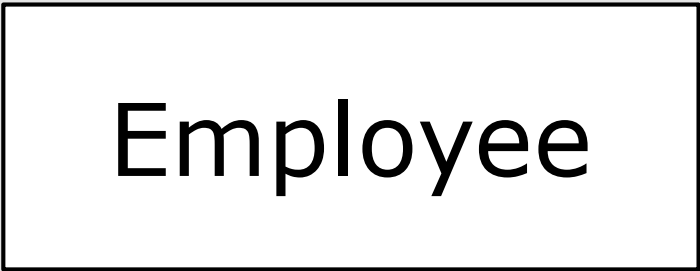
\includegraphics[width=\linewidth]{images/erd/entity.png}
            \caption{Entity Type}
            \label{fig:entity}
        \end{minipage}%
        \hspace{1cm}%
        \begin{minipage}[t]{0.4\textwidth}
            \centering
            
\includegraphics[width=\linewidth]{images/erd/weakentity.png}
            \caption{Weak Entity Type}
            \label{fig:entity-weak}
        \end{minipage}
    \end{figure}
    \item \textbf{Attributes:} A particular property that describes
an entity via a value.
    \begin{figure}[H]
        \centering
        \begin{minipage}[t]{0.4\textwidth}
            \centering
            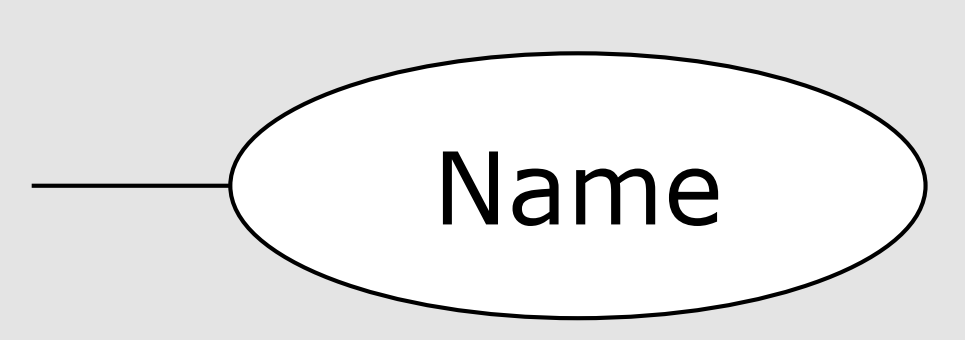
\includegraphics[width=\linewidth]{images/erd/attribute.png}
            \caption{Attribute}
            \label{fig:attribute}
        \end{minipage}%
        \hspace{1cm}%
        \begin{minipage}[t]{0.4\textwidth}
            \centering
            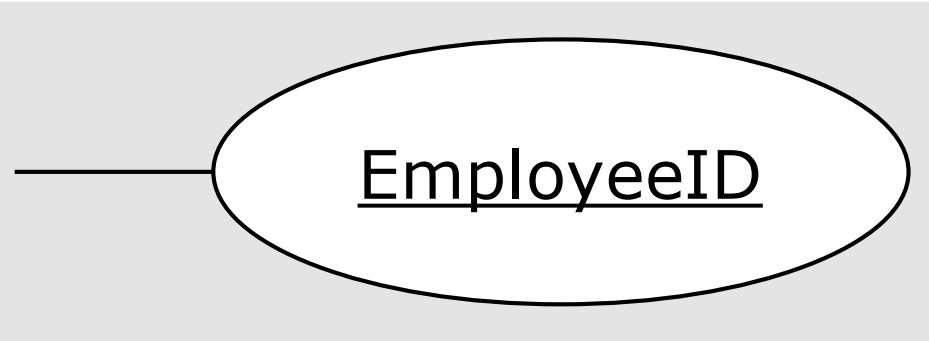
\includegraphics[width=\linewidth]{images/erd/keyattribute.png}
            \caption{Key Attribute}
            \label{fig:key-attribute}
        \end{minipage}
    \end{figure}
    \begin{figure}[H]
        \centering
        \begin{minipage}[t]{0.4\textwidth}
            \centering
            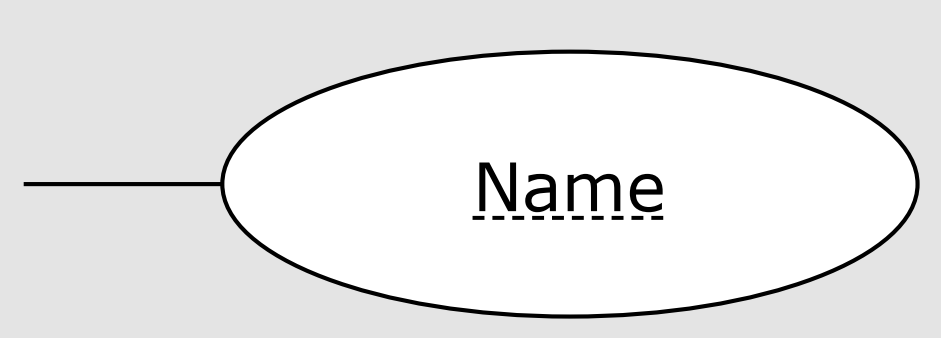
\includegraphics[width=\linewidth]{images/erd/partialattribute.png}
            \caption{Partial Key Attribute}
            \label{fig:partial-key-attribute}
        \end{minipage}%
        \hspace{1cm}%
        \begin{minipage}[t]{0.4\textwidth}
            \centering
            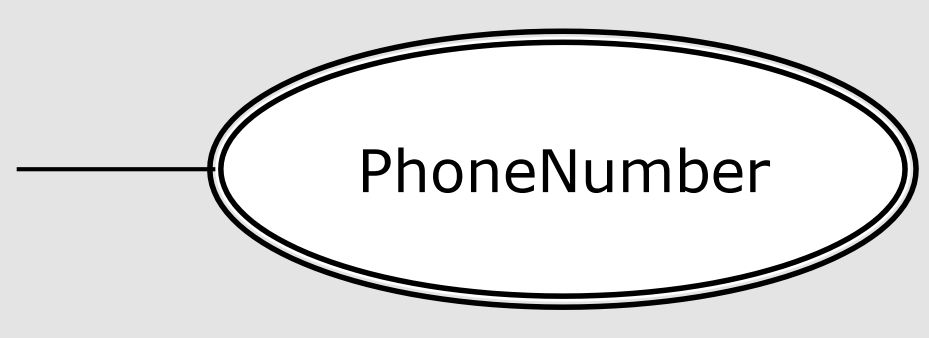
\includegraphics[width=\linewidth]{images/erd/multivaluedattribute.png}
            \caption{Multivalued Attribute}
            \label{fig:multivalued-attribute}
        \end{minipage}
    \end{figure}
    \begin{figure}[H]
        \centering
        \begin{minipage}[t]{0.4\textwidth}
            \centering
            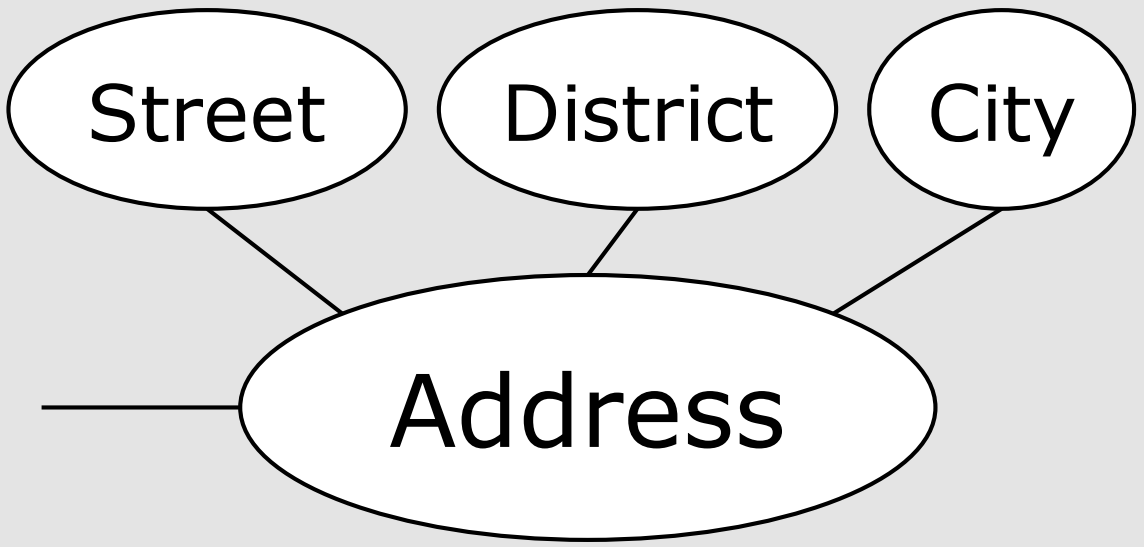
\includegraphics[width=\linewidth]{images/erd/compositeattribute.png}
            \caption{Composite Attribute}
            \label{fig:composite-attribute}
        \end{minipage}%
        \hspace{1cm}%
        \begin{minipage}[t]{0.4\textwidth}
            \centering
            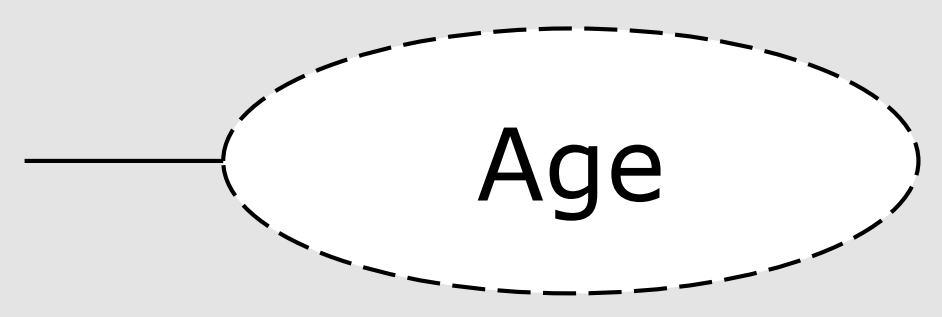
\includegraphics[width=\linewidth]{images/erd/deviredattribute.png}
            \caption{Devired Attribute}
            \label{fig:devired-attribute}
        \end{minipage}
    \end{figure}
    \item \textbf{Relationships:} A set of associations among entities.
    \begin{figure}[H]
        \centering
        \begin{minipage}[t]{0.4\textwidth}
            \centering
            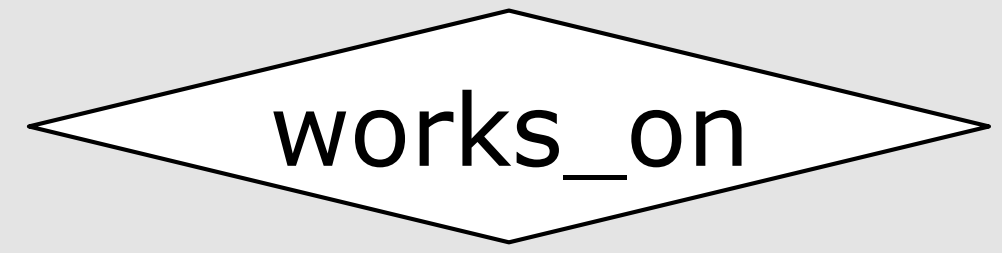
\includegraphics[width=\linewidth]{images/erd/relationship.png}
            \caption{Relationship Type}
            \label{fig:relationship}
        \end{minipage}%
        \hspace{1cm}%
        \begin{minipage}[t]{0.4\textwidth}
            \centering
            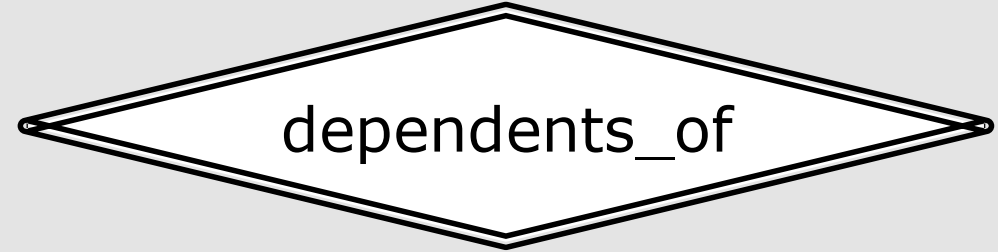
\includegraphics[width=\linewidth]{images/erd/weakrelationship.png}
            \caption{Relationship Type of Weak Entity Type}
            \label{fig:weak-relationship}
        \end{minipage}
    \end{figure}
    \item \textbf{Structural Constraints:} Limitations and rules on how entities participate in relationships, determining valid data configurations.
    \begin{itemize}
        \item \textbf{Single line:} Partial participation (optional).
        \item \textbf{Double line:} Total participation (mandatory / existence dependency).
        \item \textbf{1 and N:} Cardinality ratio (specifies 1:1, 1:N, or M:N associations).
        \item \textbf{(min, max):} Explicit lower and upper bounds of participation.
    \end{itemize}
    \begin{figure}[H]
        \centering
        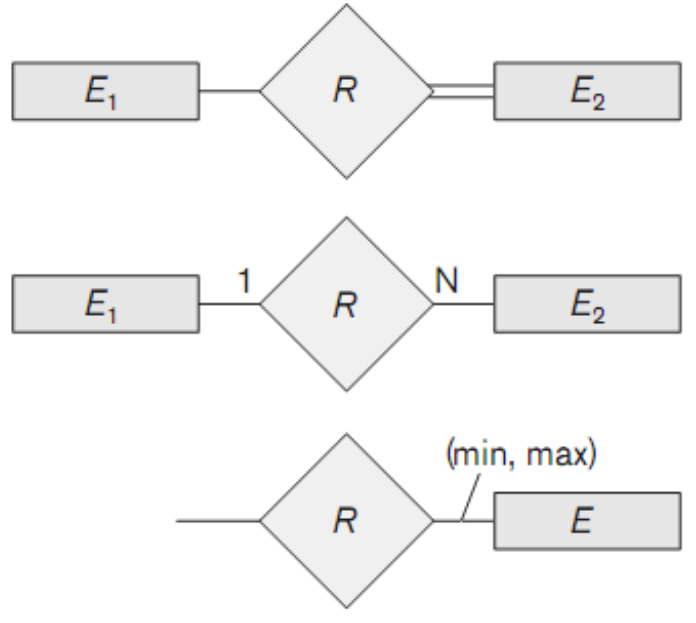
\includegraphics[width=0.45\textwidth]{images/erd/constraints.png}
        \caption{Structural Constraints on Relationship Types}
        \label{fig:structural-constraints}
    \end{figure}
\end{enumerate}







\section{Technologies}

\subsection{Python and FastAPI}

Python is a high-level, general-purpose programming language known for
its readable syntax, flexibility, and extensive ecosystem of libraries.
It supports multiple programming paradigms, including procedural,
object-oriented, and asynchronous programming, making it suitable for
developing modern backend applications and data-driven systems.

FastAPI is a modern Python web framework designed for building
high-performance RESTful APIs. It uses Python type hints and Pydantic
for request validation, data serialization, and schema definition.
FastAPI also automatically generates interactive API documentation
through OpenAPI and Swagger UI, simplifying API development, testing,
and integration.

In this system, Python and FastAPI are used to implement backend
business logic and expose API endpoints for communication between
the client application, application services, and the database.

\subsection{Uvicorn}

Uvicorn is a lightweight ASGI (Asynchronous Server Gateway Interface)
server designed to run asynchronous Python web applications.
It uses an event-driven architecture to handle concurrent connections
efficiently and supports asynchronous request processing through
Python's \texttt{async} and \texttt{await} syntax.

Unlike a web framework, Uvicorn does not define application endpoints
or business logic. Instead, it receives incoming HTTP requests,
forwards them to the ASGI application, and returns the generated
responses to clients.

In this system, Uvicorn serves as the application server for FastAPI,
allowing the backend API to receive and process HTTP requests.
It can be configured with multiple worker processes when additional
request-processing capacity is required.

\subsection{PostgreSQL}

PostgreSQL is an open-source relational database management system
that provides reliable data storage, advanced querying capabilities,
and strong transactional guarantees. It supports SQL, primary and
foreign keys, indexes, constraints, and database transactions to
maintain data consistency and integrity.

PostgreSQL follows the ACID properties of database transactions:
Atomicity, Consistency, Isolation, and Durability. These properties
help ensure that related database operations are executed reliably.
It also provides features such as indexing, concurrency control,
and extensible data types to support different application requirements.

In this system, PostgreSQL stores persistent application data,
including user information, business records, and relationships
between entities. Its transactional capabilities help maintain
data integrity when multiple users or requests access the system
concurrently.

\subsection{Nginx}

Nginx is a high-performance web server that can also function as
a reverse proxy, load balancer, and HTTP cache. It is designed to
handle a large number of concurrent connections with relatively
low resource consumption, making it suitable for production
environments.

As a reverse proxy, Nginx receives incoming client requests and
forwards them to the appropriate backend application server.
It can also handle HTTPS termination, configure request limits,
and distribute traffic among multiple application instances.
These capabilities help separate public-facing traffic management
from backend application processing.

In this system, Nginx acts as the entry point for incoming HTTP
or HTTPS requests and forwards API traffic to Uvicorn running
the FastAPI application. This configuration provides a clear
boundary between external clients and the backend services.

\subsection{Docker}

Docker is a containerization platform that packages an application
and its dependencies into a standardized container image. Containers
provide isolated execution environments while sharing the host
operating system kernel, making them generally more lightweight
than traditional virtual machines.

A Docker image defines the application environment, including
the required runtime, libraries, configuration, and application
files. A Docker container is a running instance of that image.
Using a \texttt{Dockerfile} and container configuration allows
developers to reproduce application environments consistently
across development, testing, and deployment.

In this system, Docker packages the backend application and its
runtime dependencies into containers. It can also be used to run
PostgreSQL and Nginx as separate containers, allowing the main
components to be configured, deployed, and managed independently.
Docker Compose can simplify local development by defining how
these containers interact within a shared network.

\subsection{PHP}

(PHP: Hypertext Preprocessor) is a free, open-source, general-purpose scripting language particularly suited for web development. Its scripts execute on the server, enabling the creation of dynamic and interactive web pages, and PHP can be embedded into HTML.

\subsection{Moodle}
Moodle, short for Modular Object-Oriented Dynamic Learning Environment, is a free, open-source Learning Management System (LMS) designed to support online and blended learning. It provides a platform where educators can create and manage courses, share learning materials, organize activities, assess students, and support communication between learners and teachers. Since Moodle is open source, its code can be modified and extended to meet the needs of different educational institutions. 
Moodle provides a range of built-in learning tools and supports additional functionality through plugins and themes. It can be installed on a web server managed by an institution, allowing the institution to configure and customize the system according to its requirements. These capabilities make Moodle suitable as a foundation for projects that extend an existing learning environment with additional features.

\medskip
\noindent\textbf{User Interface.} Moodle provides a web-based interface through which students, teachers, and administrators access learning and management functions. Depending on their roles and permissions, users can view courses, access learning resources, submit assignments, participate in activities, manage course content, and review grades. The appearance of a Moodle site can also be customized using themes, allowing institutions to adjust its layout and visual presentation. 

\medskip
\noindent\textbf{Database.} Moodle uses a database to store structured information required for the operation of the learning platform. This includes information about users, courses, enrollments, activities, grades, and system configuration. Moodle supports several database systems, including PostgreSQL, MySQL-compatible databases, and Microsoft SQL Server. The database stores structured records, while uploaded files are handled through Moodle's file storage system.

\medskip
\noindent\textbf{Moodledata.} The moodledata directory is used to store files and supporting data generated or managed during Moodle's operation. It includes uploaded course materials and user files, as well as temporary files, cached data, and session-related information. Unlike the database, which stores structured records, moodledata provides file storage for the Moodle site. For security, this directory should be located outside the web-accessible directory.

\medskip
\noindent\textbf{Moodle Architecture and Integration.} Moodle consists of several components that work together to provide an online learning environment. The Moodle application contains the core functionality and handles user requests, while the database stores structured information and the moodledata directory stores uploaded files and other supporting data. These components work together to support course management, learning activities, and other platform functions.

Moodle also provides mechanisms for extending its functionality and communicating with external systems. Its plugin system allows developers to add features for specific purposes, while its Web Services framework enables external applications to access supported Moodle functions through configured endpoints. These mechanisms provide possible approaches for integrating additional services into an existing Moodle environment.

Regarding plugin organization, Moodle categorizes plugins by their types, with each type corresponding to a specific functionality and directory within the platform. For example, activity modules are stored in the \texttt{mod} directory, blocks are stored in the \texttt{blocks} directory, and local plugins are stored in the \texttt{local} directory. Moodle uses a naming convention known as \textit{Frankenstyle} to uniquely identify plugin components. A component name consists of the plugin type prefix followed by the plugin name, separated by an underscore. For example, \texttt{mod\_quiz} identifies the Quiz activity module, while \texttt{block\_html} identifies the HTML block plugin. This convention provides a consistent way to identify plugins throughout the platform.

\medskip
\noindent\textbf{Moodle Community.} Moodle is supported by an international community of educators, administrators, developers, and organizations. Its official documentation, discussion forums, and plugin directory provide resources for learning, troubleshooting, and extending the platform. Developers can use Moodle's plugin system to add or customize functionality without necessarily changing the core code, making it easier to maintain extensions as the platform evolves.

\subsection{Webpack}
Webpack is a static module bundler for modern JavaScript applications. It analyzes an application's entry points and their dependencies to construct a dependency graph, then combines the required modules into one or more bundles that can be delivered to a web browser. Webpack supports different types of resources through loaders and plugins, allowing developers to configure how application files are processed during the build process.

\subsection{React App}
React is a JavaScript library for building user interfaces through reusable components. Each component represents a part of the interface and can contain its own presentation and behavior. By combining components, developers can construct larger interfaces while reusing common elements such as navigation bars, forms, buttons, tables, and dialog boxes. This component-based approach helps organize frontend code and makes interfaces easier to maintain as an application grows.

\subsection{Generative AI}
Generative Artificial Intelligence (Generative AI) refers to AI systems that generate new content in response to input instructions or contextual information. Depending on the model and application, generated content may include natural-language text, summaries, explanations, images, or other forms of output. Large Language Models (LLMs) are particularly relevant to text-based applications because they can interpret natural-language questions and produce responses in a conversational format.


\subsection{GitHub}
GitHub is a platform for hosting Git repositories and supporting collaborative software development. Git is a distributed version control system that records changes to files over time, while GitHub provides repository hosting and collaboration features around that version history. Developers can use repositories to organize source code and related project files, commits to record changes, and branches to work on separate features or fixes without directly modifying the main development branch.


\chapter{System Analysis}
\section{Functional Requirements}

This section lists the functional requirements of the system, grouped by module. Because the project extends Moodle instead of rebuilding a learning management system, each requirement states whether it is \textbf{inherited} from Moodle (configured and exposed through the new portal) or \textbf{new} (developed by the team as plugins or external services). The \textit{Phase} column indicates whether the requirement is delivered in the specialized project (Phase 1) or the graduation project (Phase 2).


\newcommand{\frtablehead}{%
\hline
\textbf{ID} & \textbf{Requirement} & \textbf{Source} & \textbf{Phase} \\ \hline}

\newenvironment{frtable}[2]{%
\small\renewcommand{\arraystretch}{1.15}
\begin{longtable}{|>{\raggedright\arraybackslash}p{0.15\textwidth}|>{\raggedright\arraybackslash}p{0.5\textwidth}|>{\centering\arraybackslash}p{0.12\textwidth}|>{\centering\arraybackslash}p{0.08\textwidth}|}
\caption{#1}\label{#2}\\
\frtablehead
\endfirsthead
\frtablehead
\endhead
}{%
\end{longtable}}

\subsection{Common user functions}
\begin{frtable}{Functional requirements: common user functions}{tab:fr-user}
FR-USR-01 & The system shall allow every user to log in with a username or email and password and shall redirect the user to the dashboard of their role (Student, Teacher, or Administrator). & Inherited & 1 \\ \hline
FR-USR-02 & The system shall allow users to log out and shall end a session automatically after a configurable period of inactivity. & Inherited & 1 \\ \hline
FR-USR-03 & The system shall allow users to view their profile and update editable fields (phone number, avatar, personal email), while keeping identity fields (user ID, full name, role) read-only. & Inherited & 1 \\ \hline
FR-USR-04 & The system shall restrict every function and every piece of data according to the user's role and course enrollment (role-based access control). & New & 1 \\ \hline
FR-USR-05 & The system shall display in-app notifications (e.g., new materials, deadlines, risk warnings) to the users concerned. & Inherited & 1 \\ \hline
\end{frtable}

\subsection{Student module}
\begin{frtable}{Functional requirements: student module}{tab:fr-student}
FR-STU-01 & The system shall allow students to browse, search, and filter the catalog of available courses and view course details (description, credits, prerequisites, lecturer, schedule). & Inherited & 1 \\ \hline
FR-STU-02 & The system shall allow students to register for a course section during the registration period, checking prerequisites, credit limits, seat availability, and schedule conflicts. & Inherited & 1 \\ \hline
FR-STU-03 & The system shall allow students to view the list of courses they are enrolled in. & Inherited & 1 \\ \hline
FR-STU-04 & The system shall allow students to view and download the learning materials of their enrolled courses. & Inherited & 1 \\ \hline
FR-STU-05 & The system shall allow students to take online quizzes within the configured time window and attempt limit. & Inherited & 1 \\ \hline
FR-STU-06 & The system shall allow students to submit assignments as files or online text before the deadline and shall mark late submissions. & Inherited & 1 \\ \hline
FR-STU-07 & The system shall allow students to view their published grades and the feedback given by teachers. & Inherited & 1 \\ \hline
FR-STU-08 & The system shall display each student's learning progress (completed and remaining activities) for each enrolled course. & Inherited & 1 \\ \hline
FR-STU-09 & The system shall display a calendar of classes, assignment deadlines, and exam dates for the student's enrolled courses. & Inherited & 1 \\ \hline
FR-STU-10 & The system shall allow students to communicate with teachers and classmates through course forums and messages. & Inherited & 1 \\ \hline
\end{frtable}

\subsection{Teacher module}
\begin{frtable}{Functional requirements: teacher module}{tab:fr-teacher}
FR-TEA-01 & The system shall allow teachers to view the list of courses they are assigned to teach and open each course's home page. & Inherited & 1 \\ \hline
FR-TEA-02 & The system shall allow teachers to view, search, and filter the roster of enrolled students, including each student's last access time. & Inherited & 1 \\ \hline
FR-TEA-03 & The system shall allow teachers to upload learning materials (PDF, DOCX, PPTX, links) to course sections. & Inherited & 1 \\ \hline
FR-TEA-04 & The system shall allow teachers to create, edit, and delete quizzes, including time windows, attempt limits, and questions from the question bank. & Inherited & 1 \\ \hline
FR-TEA-05 & The system shall allow teachers to create, edit, and delete assignments with submission dates, deadlines, and file limits. & Inherited & 1 \\ \hline
FR-TEA-06 & The system shall allow teachers to grade quizzes and assignments and give feedback to students. & Inherited & 1 \\ \hline
FR-TEA-07 & The system shall allow teachers to view the academic performance of each student and of the whole class. & Inherited & 1 \\ \hline
\end{frtable}

\subsection{Administrator module}
\begin{frtable}{Functional requirements: administrator module}{tab:fr-admin}
FR-ADM-01 & The system shall allow administrators to create, update, and deactivate user accounts, individually or by bulk import. & Inherited & 1 \\ \hline
FR-ADM-02 & The system shall allow administrators to assign and revoke roles (Student, Teacher, Administrator). & Inherited & 1 \\ \hline
FR-ADM-03 & The system shall allow administrators to create, update, and delete courses. & Inherited & 1 \\ \hline
FR-ADM-04 & The system shall allow administrators to create classes and sections, assign teachers to them, and assign students to them. & Inherited & 1 \\ \hline
FR-ADM-05 & The system shall allow administrators to review course registrations and manage class schedules. & Inherited & 1 \\ \hline
FR-ADM-06 & The system shall allow administrators to send notifications to selected users, classes, or all users. & Inherited & 1 \\ \hline
FR-ADM-07 & The system shall allow administrators to manage system configuration, including the settings of the AI features (language model provider, risk thresholds, synchronization schedule). & New & 1 \\ \hline
FR-ADM-08 & The system shall allow administrators to monitor the AI services, including request counts, latency, error rates, and language model token usage. & New & 2 \\ \hline
\end{frtable}

\subsection{Data integration and document processing}
\begin{frtable}{Functional requirements: data integration and document processing}{tab:fr-integration}
FR-INT-01 & The system shall synchronize users, courses, enrollments, grades, submissions, and activity logs from Moodle to the extension services through Moodle Web Services or scheduled database extraction, without modifying the Moodle core. & New & 1 \\ \hline
FR-INT-02 & The system shall route every request from the portal to the AI Service through the backend gateway, which authenticates the user and checks permissions before forwarding the request. & New & 1 \\ \hline
FR-INT-03 & The system shall automatically convert newly uploaded course materials (PDF, DOCX, PPTX) into structured Markdown text that keeps headings and page numbers. & New & 1 \\ \hline
FR-INT-04 & The system shall split the converted text into chunks, compute their embeddings, and store them in the vector database together with metadata (course, section, file, page). & New & 1 \\ \hline
FR-INT-05 & The system shall re-index a document when it is updated and remove its chunks when it is deleted from the course. & New & 1 \\ \hline
FR-INT-06 & The system shall extract text from scanned documents using optical character recognition (OCR). & New & 2 \\ \hline
\end{frtable}

\subsection{AI learning assistant (RAG chatbot)}
\begin{frtable}{Functional requirements: AI learning assistant}{tab:fr-chatbot}
FR-CHAT-01 & The system shall allow students and teachers to ask questions in natural language (Vietnamese or English) within the context of a course. & New & 1 \\ \hline
FR-CHAT-02 & The system shall retrieve context only from the materials of courses the user is enrolled in or teaches. & New & 1 \\ \hline
FR-CHAT-03 & The system shall generate answers grounded in the retrieved context and attach citations (file name and page or section) to each answer. & New & 1 \\ \hline
FR-CHAT-04 & The system shall state explicitly that it cannot find the answer when no sufficiently relevant context is retrieved, instead of generating unsupported content. & New & 1 \\ \hline
FR-CHAT-05 & The system shall stream answers to the interface progressively as they are generated. & New & 1 \\ \hline
FR-CHAT-06 & The system shall store chat sessions, messages, and citations so that users can review their conversation history and ask follow-up questions in context. & New & 1 \\ \hline
FR-CHAT-07 & The system shall allow users to open the cited source document at the referenced page. & New & 2 \\ \hline
FR-CHAT-08 & The system shall allow users to limit the search scope to a specific chapter or document and to rate answers (like or dislike). & New & 2 \\ \hline
FR-CHAT-09 & The system shall combine semantic (vector) search with keyword (BM25) search and re-rank the retrieved chunks to improve answer accuracy. & New & 2 \\ \hline
\end{frtable}

\subsection{Academic early warning}
\begin{frtable}{Functional requirements: academic early warning}{tab:fr-warning}
FR-RISK-01 & The system shall periodically compute risk indicators for each enrolled student, including days since last access, activity completion rate, recent assessment scores and their trend, submission delays, and number of missing submissions. & New & 1 \\ \hline
FR-RISK-02 & The system shall flag at-risk students using configurable threshold rules (e.g., no access for more than 7 days, completion rate below 50\%, latest score below 5.0 or missing submission). & New & 1 \\ \hline
FR-RISK-03 & The system shall predict each student's probability of failing or withdrawing from a course with a machine learning model (gradient boosted trees) trained on historical learning data. & New & 2 \\ \hline
FR-RISK-04 & The system shall classify each student into a risk level (High, Medium, or Low) based on the computed rules or predicted probability. & New & 1 \\ \hline
FR-RISK-05 & The system shall explain each warning by listing its main contributing factors in plain language (e.g., ``Inactive for 14 days'', ``Quiz score dropped 25\% below the student's average''), computed with SHAP in Phase 2. & New & 1 \\ \hline
FR-RISK-06 & The system shall display to teachers a list of at-risk students for each course, which can be sorted and filtered by risk level, together with a detailed view of each student's indicators and risk history. & New & 1 \\ \hline
FR-RISK-07 & The system shall display to each student only their own warnings, together with suggested actions (e.g., materials to review, assignments to submit). & New & 1 \\ \hline
FR-RISK-08 & The system shall allow teachers to send a reminder message to an at-risk student, optionally starting from a draft generated by the language model from the warning factors. & New & 2 \\ \hline
\end{frtable}

\subsection{Course recommendation}
\begin{frtable}{Functional requirements: course recommendation}{tab:fr-recommendation}
FR-REC-01 & The system shall recommend suitable courses to students based on their major, completed courses, prerequisites, and academic results, and shall give the reason for each recommendation. & New & 2 \\ \hline
\end{frtable}

\section{Non-functional Requirements}

The non-functional requirements below are stated with measurable targets wherever possible, so that they can be verified during testing. Because the system is evaluated at a small scale (a few courses and sample users, see Section 1.3), the targets are set for that scale and for the limited hardware available to the team.

\newcommand{\nfrtablehead}{%
\hline
\textbf{ID} & \textbf{Category} & \textbf{Requirement} \\ \hline}

\newenvironment{nfrtable}[2]{%
\small\renewcommand{\arraystretch}{1.15}
\begin{longtable}{|>{\raggedright\arraybackslash}p{0.17\textwidth}|>{\raggedright\arraybackslash}p{0.17\textwidth}|>{\raggedright\arraybackslash}p{0.56\textwidth}|}
\caption{#1}\label{#2}\\
\nfrtablehead
\endfirsthead
\nfrtablehead
\endhead
}{%
\end{longtable}}

\subsection{Performance and scalability}
\begin{nfrtable}{Non-functional requirements: performance and scalability}{tab:nfr-performance}
NFR-PER-01 & Response time & Non-AI pages and API calls of the portal shall respond within 2 seconds (95th percentile) with 100 concurrent users. \\ \hline
NFR-PER-02 & AI response time & The chatbot shall display the first part of a streamed answer within 3 seconds and complete answers of up to about 300 words within 15 seconds (95th percentile). \\ \hline
NFR-PER-03 & Dashboard load & The at-risk student dashboard of a class of up to 200 students shall load within 3 seconds, because risk scores are computed in advance and not at request time. \\ \hline
NFR-PER-04 & Batch processing & Risk indicators and scores for all test courses shall be recomputed by a scheduled job (at least daily) that finishes within 30 minutes. \\ \hline
NFR-PER-05 & Asynchronous processing & Document conversion, indexing, and model inference shall run asynchronously through a message queue, so that uploading a file or requesting an analysis never blocks the user interface; a 50-page PDF shall be searchable within 5 minutes of upload. \\ \hline
NFR-SCA-01 & Scalability & The backend gateway and the AI Service shall be stateless and packaged as containers, so that more instances can be added behind the reverse proxy to handle a higher load without code changes. \\ \hline
\end{nfrtable}

\subsection{Reliability and availability}
\begin{nfrtable}{Non-functional requirements: reliability and availability}{tab:nfr-reliability}
NFR-REL-01 & Fault isolation & A failure of the AI Service or the language model provider shall not affect the core LMS functions; the portal shall show a clear temporary error for the AI features only. \\ \hline
NFR-REL-02 & Graceful degradation & When the warning model cannot run, the system shall display the most recently computed results together with their computation time, or fall back to the threshold rules. \\ \hline
NFR-REL-03 & Data consistency & Data synchronization from Moodle shall be idempotent and resumable: re-running a synchronization job shall not create duplicate records. \\ \hline
NFR-REL-04 & Backup & The databases (Moodle, application, and vector database) shall be backed up at least daily, and a backup shall be restorable within 2 hours. \\ \hline
\end{nfrtable}

\subsection{Security and privacy}
\begin{nfrtable}{Non-functional requirements: security and privacy}{tab:nfr-security}
NFR-SEC-01 & Transport security & All communication between clients and the system, and between public services, shall use HTTPS (TLS 1.2 or higher). \\ \hline
NFR-SEC-02 & Authentication & Every API request to the gateway and the AI Service shall carry a valid access token; tokens shall expire after a configurable period. \\ \hline
NFR-SEC-03 & Authorization & Role and enrollment checks shall be enforced on the server side for every request: a student can only access their own data and enrolled courses, and a teacher can only access the courses they teach. \\ \hline
NFR-SEC-04 & Credential handling & User passwords shall be managed only by Moodle and never stored by the extension services; API keys and secrets shall be stored in environment variables or a secret store, never in source code. \\ \hline
NFR-SEC-05 & Abuse prevention & The chatbot shall limit each user to a configurable number of requests per minute (default 20), validate all inputs, and apply instructions that prevent prompt injection from overriding system rules. \\ \hline
NFR-PRI-01 & Data minimization & Only the question and the retrieved course text shall be sent to an external language model; names, student IDs, emails, and grades shall not be included in prompts, and student identifiers shall be pseudonymized. \\ \hline
NFR-PRI-02 & Warning visibility & Risk warnings of a student shall be visible only to that student, the teachers of the course, and administrators. \\ \hline
NFR-AUD-01 & Auditability & The system shall log administrative actions and AI requests (user, course, time, latency, token usage, status) for monitoring and auditing, without storing passwords or access tokens. \\ \hline
\end{nfrtable}

\subsection{Maintainability, extensibility, and portability}
\begin{nfrtable}{Non-functional requirements: maintainability, extensibility, and portability}{tab:nfr-maintainability}
NFR-MNT-01 & Upgrade safety & The Moodle core shall not be modified; all extensions shall be implemented as Moodle plugins or external services, so that Moodle can be upgraded independently. \\ \hline
NFR-MNT-02 & Modularity & The portal, backend gateway, data-processing service, and AI Service shall communicate only through documented REST APIs (OpenAPI specification), so that each component can be developed, tested, and deployed independently. \\ \hline
NFR-MNT-03 & Extensibility & The language model provider, embedding model, and warning model shall be replaceable through configuration and model versioning, without changing business logic. \\ \hline
NFR-MNT-04 & Code quality & Source code shall be managed with Git using feature branches merged into a development branch through pull requests; core business logic and AI pipelines shall have automated tests. \\ \hline
NFR-POR-01 & Portability & The whole system (Moodle, databases, backend gateway, AI Service, and portal) shall be started with a single Docker Compose configuration in development and test environments. \\ \hline
\end{nfrtable}

\subsection{Usability and compatibility}
\begin{nfrtable}{Non-functional requirements: usability and compatibility}{tab:nfr-usability}
NFR-USA-01 & Language & The interface shall support Vietnamese as the primary language and English as a secondary language. \\ \hline
NFR-USA-02 & Clarity & Risk warnings shall be presented with a color-coded level (red, amber, green) and their contributing factors in plain language, so that users without technical knowledge can understand why a student was flagged. \\ \hline
NFR-USA-03 & Responsiveness & The portal shall be usable on screens from 360 pixels wide (mobile phones) to desktop monitors. \\ \hline
NFR-USA-04 & Learnability & A new user shall be able to ask the chatbot a question or open the at-risk student list without training, within three clicks from their dashboard. \\ \hline
NFR-COM-01 & Browser support & The portal shall work on the two latest major versions of Google Chrome, Microsoft Edge, and Mozilla Firefox. \\ \hline
NFR-COM-02 & Platform & The extensions shall be compatible with Moodle 5.x and PostgreSQL. \\ \hline
\end{nfrtable}

\subsection{Quality of AI components}
\begin{nfrtable}{Non-functional requirements: quality of AI components}{tab:nfr-ai}
NFR-AI-01 & Retrieval quality & On a test set of at least 100 questions built by the team from course materials, the relevant chunk shall be among the top 5 retrieved results (Recall@5) for at least 80\% of the questions. \\ \hline
NFR-AI-02 & Answer faithfulness & Answers shall reach a faithfulness score of at least 0.8 (RAGAS), and every answer shall either cite at least one source or state that no answer was found. \\ \hline
NFR-AI-03 & Warning effectiveness & Evaluated on held-out course presentations, the warning model shall reach a recall of at least 0.75 for the at-risk class when about 40\% of the course has elapsed, and a higher PR-AUC than the logistic regression baseline. \\ \hline
NFR-AI-04 & Explainability & Every risk prediction shall include its top three contributing factors, and the displayed factors shall be consistent with the model's SHAP values. \\ \hline
NFR-AI-05 & Fairness & The difference in model performance between demographic groups (e.g., gender, region) shall be measured (ABROCA) and reported; demographic attributes shall not be used as input features. \\ \hline
NFR-AI-06 & Human oversight & AI outputs shall be presented as decision support only; the system shall not automatically take academic decisions (such as grading or penalties) based on them. \\ \hline
\end{nfrtable}

\section{Use case}
\subsection{System Actors}

{
\renewcommand{\arraystretch}{1.2}
\begin{longtable}{|>{\bfseries\raggedright\arraybackslash}p{0.2\textwidth}|>{\raggedright\arraybackslash}p{0.68\textwidth}|}
\caption{System actors}\label{tab:system-actors}\\
\hline
\textbf{Actor} & \textbf{Description} \\ \hline
\endfirsthead
\hline
\textbf{Actor} & \textbf{Description} \\ \hline
\endhead
User & Abstract actor representing any authenticated person using the system. It owns the common use cases Login, Logout, and Update Profile, which are inherited by all concrete human actors. \\ \hline
Student & Learner enrolled in one or more courses. Browses and registers for courses, accesses learning materials, takes quizzes, submits assignments, tracks progress, asks the AI assistant questions about course materials, and views personal learning risk warnings. \\ \hline
Teacher & Lecturer assigned to teach courses. Manages course materials, quizzes, and assignments, monitors enrolled students, and reviews at-risk students together with the explanations produced by the warning model. \\ \hline
Administrator & Staff member responsible for operating the system. Manages user accounts and roles, courses, classes and schedules, notifications, and system configuration. \\ \hline
AI Service & Supporting system actor that answers course-related questions using Retrieval-Augmented Generation and computes academic risk scores with their explanations. It is invoked by the backend and never acts on its own initiative. \\ \hline
\end{longtable}
}

\subsection{System use case diagram}

\subsubsection{System use case}

\begin{figure}[H]
    \centering
    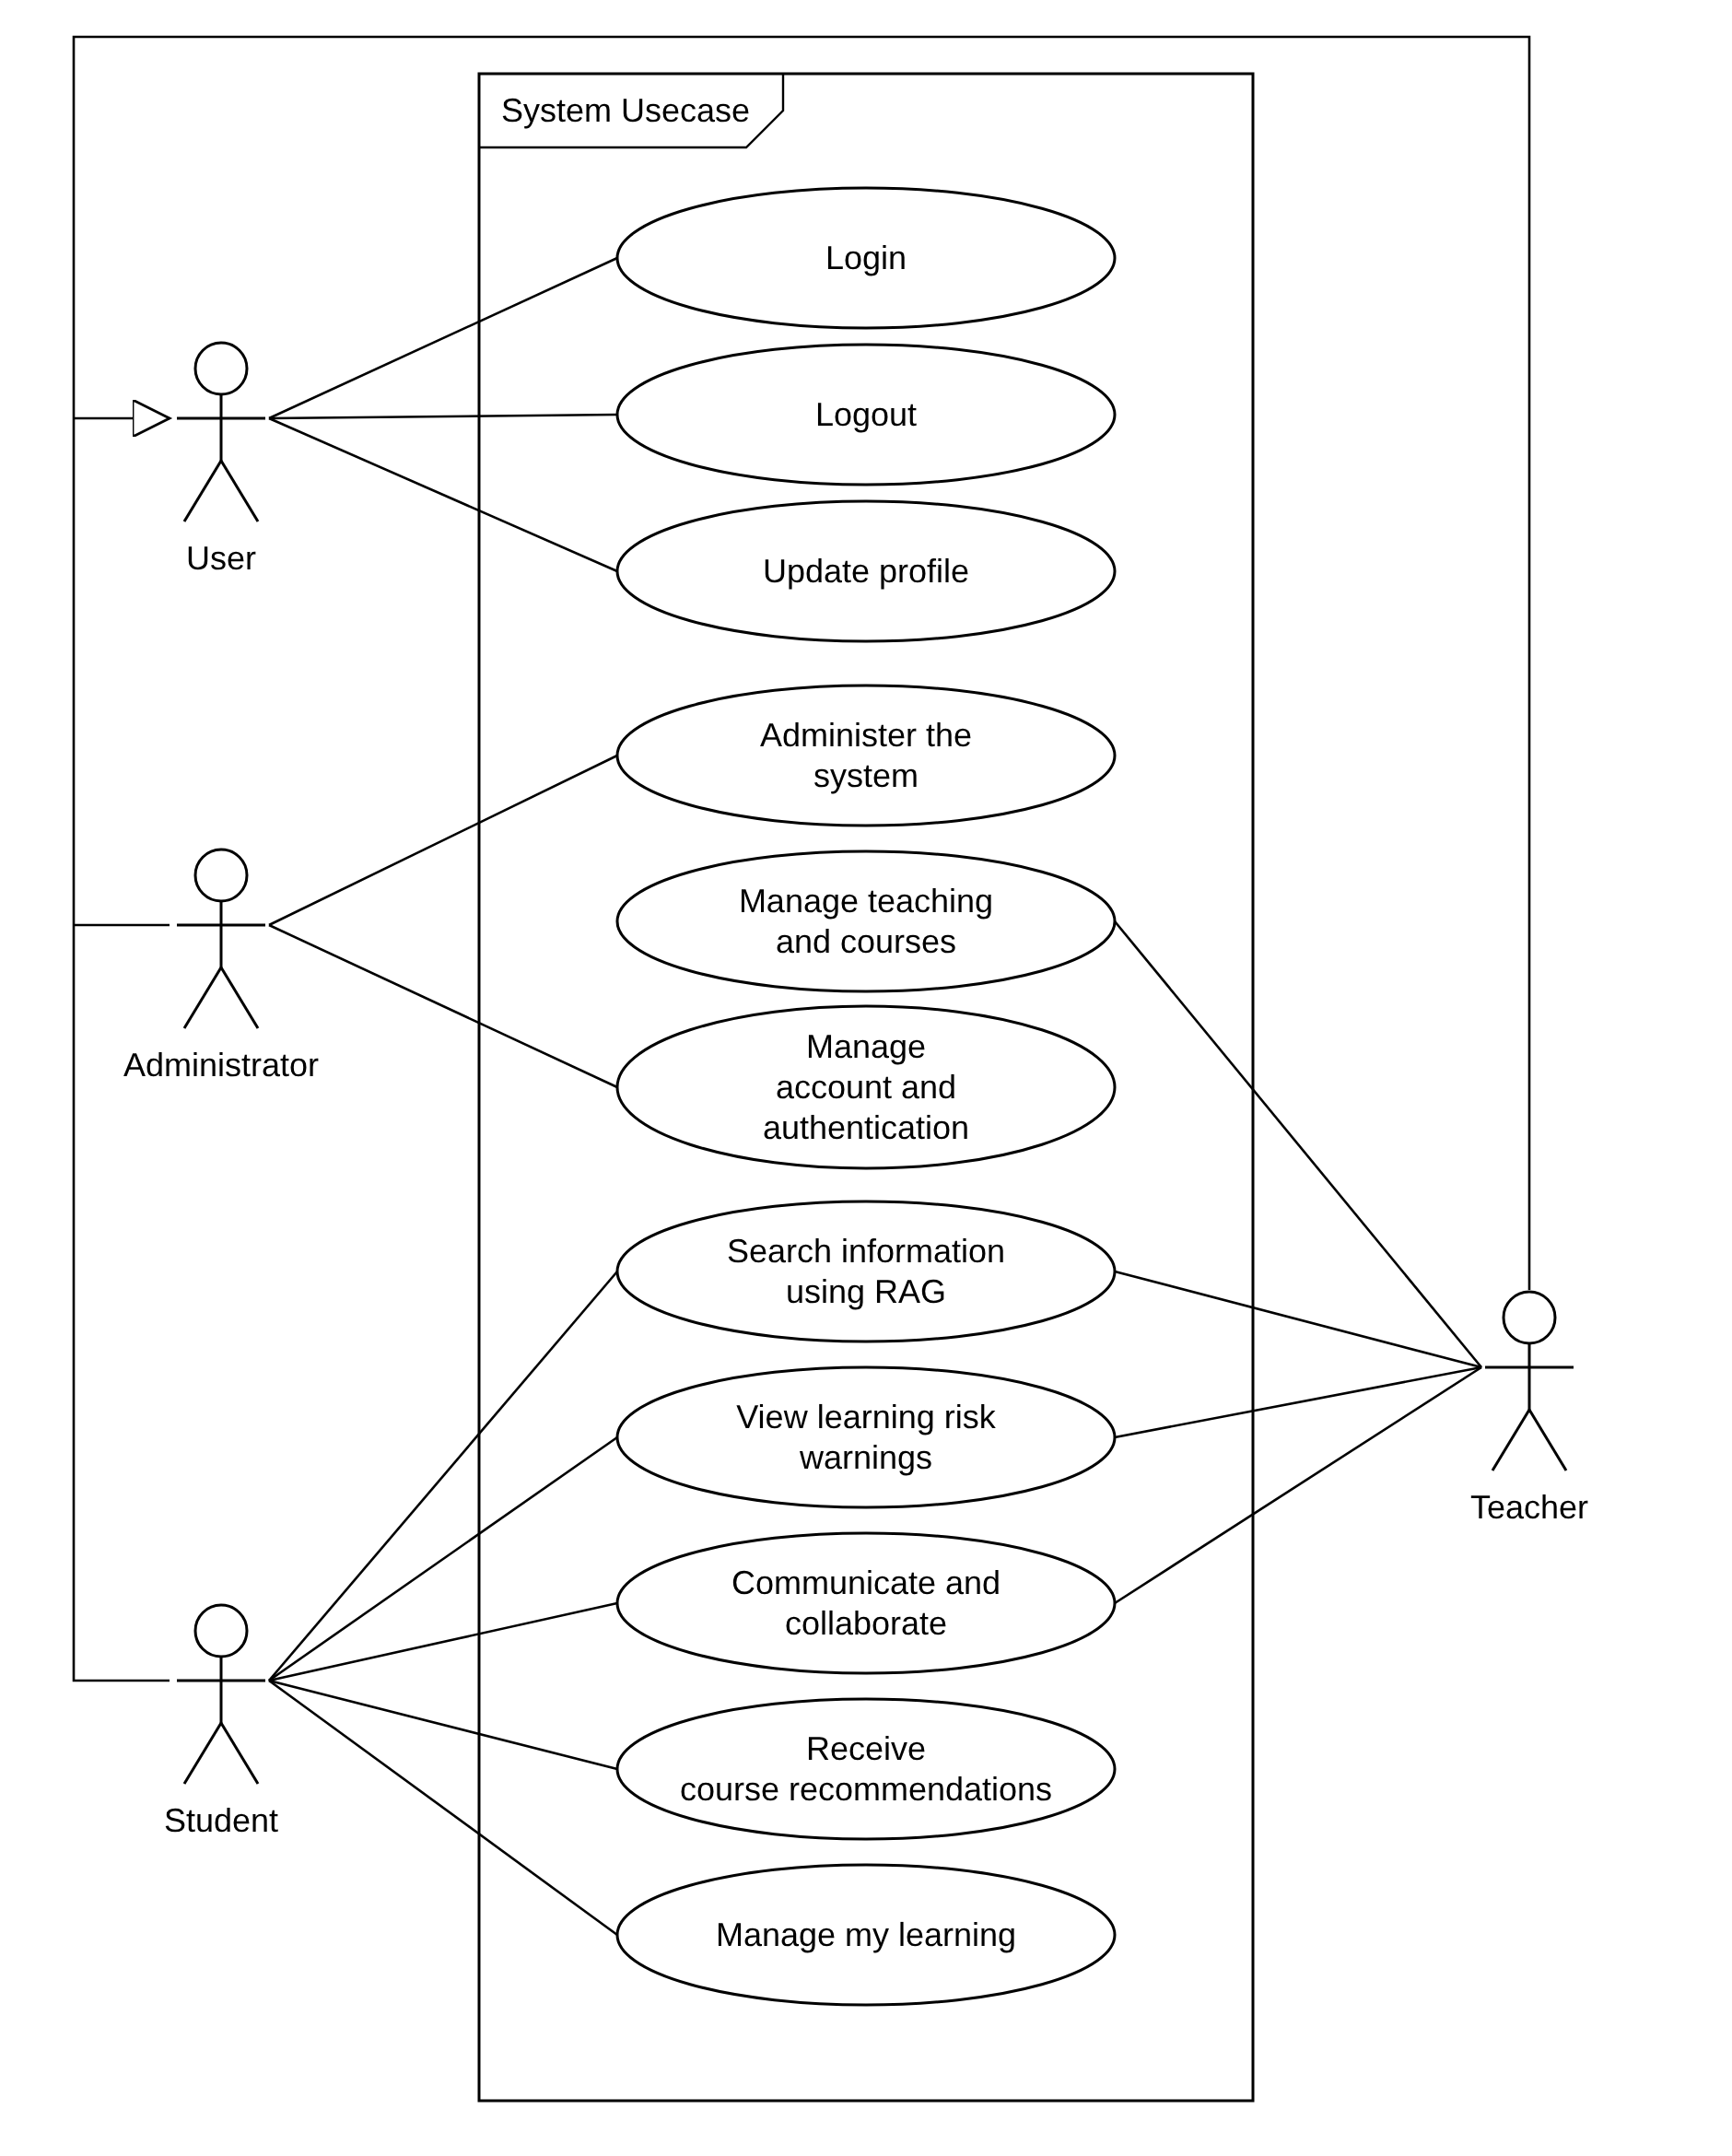
\includegraphics[width=0.7\textwidth, height=0.7\textheight, keepaspectratio]{images/usecase/system_usecase.png}
    \caption{System Use Case Diagram}
    \label{fig:system-usecase}
\end{figure}

{
\renewcommand{\arraystretch}{1.1}
\setlength{\tabcolsep}{8pt}
\begin{longtable}{|>{\bfseries\raggedright\arraybackslash}p{0.205\textwidth}|>{\raggedright\arraybackslash}p{0.685\textwidth}|}
\hline
Use-case ID & UC-USR-01 \\ \hline
Use-case name & Login \\ \hline
Author & Nguyen Manh Tri Minh \\ \hline
Description & Allows a user (Student, Teacher, or Administrator) to authenticate and access the features permitted by their role. \\ \hline
Actor & User (Student, Teacher, Administrator) \\ \hline
Trigger & The user opens the login page of the system portal. \\ \hline
Precondition &
1. The user has a valid, active account in the system. \par
2. The user is not currently logged in. \\ \hline
Postcondition & The user is authenticated, a secure session (access token) is issued, and the user can access system features according to their role. \\ \hline
Normal Flow &
1. The user enters their credentials (username or email and password). \par
2. The user submits the login form. \par
3. The system forwards the credentials to the authentication service and validates them against the user's account. \par
4. The system retrieves the user's role and permissions. \par
5. The system creates a secure session and issues an access token. \par
6. The system redirects the user to the dashboard corresponding to their role (student, teacher, or administrator dashboard). \\ \hline
Alternative Flow &
\textbf{A1: Valid session already exists} \par
1. At step 1, the system detects a valid, unexpired session for the user. \par
2. The system skips the login form and redirects the user directly to their dashboard. \\ \hline
Exception Flow &
\textbf{E1: Invalid credentials} \par
1. At step 3 of the normal flow, the credentials do not match any account. \par
2. The system rejects the login attempt, displays an error message, and prompts the user to try again. \par\vspace{4pt}
\textbf{E2: Account locked or suspended} \par
1. At step 3 of the normal flow, the system detects that the account is locked or suspended. \par
2. The system denies access and displays a message asking the user to contact the administrator. \par\vspace{4pt}
\textbf{E3: Authentication service unavailable} \par
1. At step 3 of the normal flow, the authentication service does not respond. \par
2. The system displays a temporary service error and allows the user to retry later. \\ \hline
\end{longtable}
}

{
\renewcommand{\arraystretch}{1.1}
\setlength{\tabcolsep}{8pt}
\begin{longtable}{|>{\bfseries\raggedright\arraybackslash}p{0.205\textwidth}|>{\raggedright\arraybackslash}p{0.685\textwidth}|}
\hline
Use-case ID & UC-USR-02 \\ \hline
Use-case name & Logout \\ \hline
Author & Nguyen Manh Tri Minh \\ \hline
Description & Allows a user to securely terminate their active session and leave the system. \\ \hline
Actor & User (Student, Teacher, Administrator) \\ \hline
Trigger & The user selects the logout function from the navigation menu. \\ \hline
Precondition & The user is currently logged into the system. \\ \hline
Postcondition & The user's session is terminated and the access token can no longer be used. \\ \hline
Normal Flow &
1. The user clicks the logout button. \par
2. The system invalidates the active session and clears the authentication tokens stored on the client. \par
3. The system redirects the user to the login page. \\ \hline
Alternative Flow &
\textbf{A1: Automatic logout after inactivity} \par
1. The user remains inactive for longer than the configured session timeout. \par
2. The system invalidates the session automatically. \par
3. On the next request, the system redirects the user to the login page. \\ \hline
Exception Flow &
\textbf{E1: Session already expired} \par
1. At step 2 of the normal flow, the system detects that the session has already expired. \par
2. The system redirects the user to the login page without displaying an error. \\ \hline
\end{longtable}
}

{
\renewcommand{\arraystretch}{1.1}
\setlength{\tabcolsep}{8pt}
\begin{longtable}{|>{\bfseries\raggedright\arraybackslash}p{0.205\textwidth}|>{\raggedright\arraybackslash}p{0.685\textwidth}|}
\hline
Use-case ID & UC-USR-03 \\ \hline
Use-case name & Update Profile \\ \hline
Author & Nguyen Manh Tri Minh \\ \hline
Description & Allows a user to view and update the editable fields of their personal profile, such as phone number, avatar, and personal email. Identity fields managed by the university (user ID, full name, role) are read-only. \\ \hline
Actor & User (Student, Teacher, Administrator) \\ \hline
Trigger & The user selects the option to view or edit their personal profile. \\ \hline
Precondition & The user is authenticated and logged into the system. \\ \hline
Postcondition & The updated profile information is saved and reflected throughout the system. \\ \hline
Normal Flow &
1. The user opens the profile page. \par
2. The system displays the current profile information, with editable fields enabled and identity fields shown as read-only. \par
3. The user updates the editable fields (e.g., phone number, avatar, personal email). \par
4. The user submits the form. \par
5. The system validates the data formats and checks that no read-only field has been changed. \par
6. The system saves the updated information. \par
7. The system confirms that the profile has been updated successfully. \\ \hline
Alternative Flow &
\textbf{A1: Cancel editing} \par
1. At step 3 or 4, the user selects ``Cancel''. \par
2. The system discards the changes and displays the unchanged profile. \\ \hline
Exception Flow &
\textbf{E1: Invalid data format} \par
1. At step 5 of the normal flow, a field contains malformed data (e.g., an invalid email address or an unsupported image format). \par
2. The system highlights the invalid field and requests correction; the profile is not updated. \par\vspace{4pt}
\textbf{E2: Save failure} \par
1. At step 6 of the normal flow, the system fails to save the changes. \par
2. The system displays an error message and keeps the previous profile information. \\ \hline
\end{longtable}
}


\subsubsection{Student use case}

\begin{figure}[H]
    \centering
    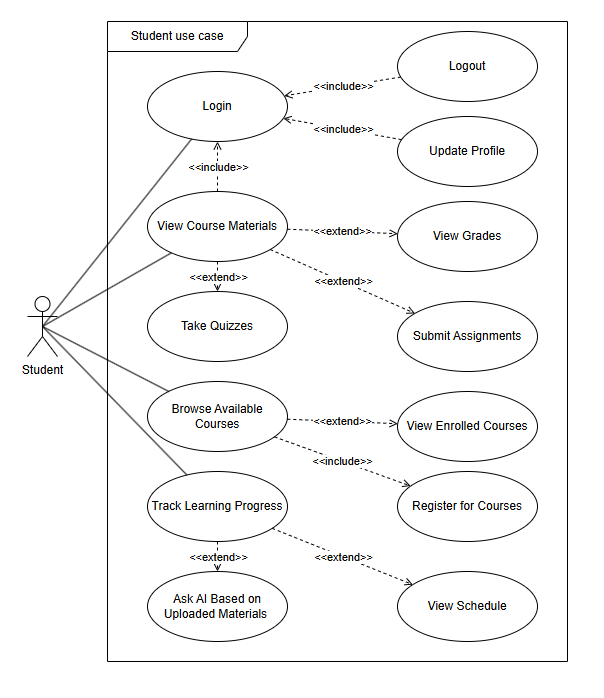
\includegraphics[width=0.5\textwidth, height=0.5\textheight, keepaspectratio]{images/usecase/student-usecase.png}
    \caption{Student Use Case Diagram}
    \label{fig:student-usecase}
\end{figure}


{
\renewcommand{\arraystretch}{1.1}
\setlength{\tabcolsep}{8pt}
\begin{longtable}{|>{\bfseries\raggedright\arraybackslash}p{0.205\textwidth}|>{\raggedright\arraybackslash}p{0.70\textwidth}|}
\hline
Use-case ID & UC-STU-01 \\ \hline
Use-case name & Login \\ \hline
Author & Dinh Cao Thien Loc \\ \hline
Description & Allows the student to authenticate and log into the system to access their personal dashboard and academic features. \\ \hline
Actor & Student \\ \hline
Trigger & The Student accesses the system's login portal. \\ \hline
Precondition &
1. The Student has a valid, active account in the system. \par
2. The Student is not currently logged in. \\ \hline
Postcondition & The Student is authenticated and can access system features according to their role. \\ \hline
Normal Flow &
1. The Student enters their credentials (e.g., username/email and password). \par
2. The Student submits the login form. \par
3. The system validates the entered credentials against the database. \par
4. If validation succeeds, the system authenticates the Student and generates a secure session. \par
5. The system redirects the Student to the student dashboard. \\ \hline
Alternative Flow & N/A. \\ \hline
Exception Flow &
\textbf{E1: Invalid credentials} \par
1. At step 3 of the normal flow, the credentials do not match the database. \par
2. The system rejects the login attempt, displays an error message, and prompts the Student to try again. \par\vspace{4pt}
\textbf{E2: Account locked or suspended} \par
1. At step 3 of the normal flow, the system detects the account is locked. \par
2. The system denies access and displays a contact support message. \\ \hline
\end{longtable}
}

{
\renewcommand{\arraystretch}{1.1}
\setlength{\tabcolsep}{8pt}
\begin{longtable}{|>{\bfseries\raggedright\arraybackslash}p{0.205\textwidth}|>{\raggedright\arraybackslash}p{0.70\textwidth}|}
\hline
Use-case ID & UC-STU-02 \\ \hline
Use-case name & Logout \\ \hline
Author & Dinh Cao Thien Loc \\ \hline
Description & Allows the student to securely terminate their active session and leave the system. \\ \hline
Actor & Student \\ \hline
Trigger & The Student selects the logout function from the navigation menu. \\ \hline
Precondition & The Student is currently logged into the system. \\ \hline
Postcondition & The Student's session is completely terminated. \\ \hline
Normal Flow &
1. The Student clicks the logout button. \par
2. The system terminates the active user session and clears authentication tokens. \par
3. The system redirects the Student to the login page or public homepage. \\ \hline
Alternative Flow & N/A. \\ \hline
Exception Flow &
\textbf{E1: Session already expired} \par
1. At step 2 of the normal flow, the system detects the session has already expired. \par
2. The system safely redirects the Student to the login page without error. \\ \hline
\end{longtable}
}

{
\renewcommand{\arraystretch}{1.1}
\setlength{\tabcolsep}{8pt}
\begin{longtable}{|>{\bfseries\raggedright\arraybackslash}p{0.205\textwidth}|>{\raggedright\arraybackslash}p{0.70\textwidth}|}
\hline
Use-case ID & UC-STU-03 \\ \hline
Use-case name & Update Profile \\ \hline
Author & Dinh Cao Thien Loc \\ \hline
Description & Allows the student to modify and update allowable personal information such as phone number, avatar, and personal email. \\ \hline
Actor & Student \\ \hline
Trigger & The Student selects the option to edit their personal profile. \\ \hline
Precondition & The Student is authenticated and logged into the system. \\ \hline
Postcondition & The Student's updated profile information is saved and reflected in the system. \\ \hline
Normal Flow &
1. The Student opens the profile management section. \par
2. The system displays the current profile information in an editable form. \par
3. The Student updates allowable fields (e.g., phone number, avatar, personal email). \par
4. The Student submits the updated form. \par
5. The system validates the data formats and checks for any prohibited changes. \par
6. The system saves the updated information to the database. \par
7. The system confirms that the profile has been updated successfully. \\ \hline
Alternative Flow & N/A. \\ \hline
Exception Flow &
\textbf{E1: Invalid data format} \par
1. At step 5 of the normal flow, the user inputs malformed data (e.g., malformed email). \par
2. The system identifies the problem, highlights the field, and requests correction; the profile is not updated. \\ \hline
\end{longtable}
}

{
\renewcommand{\arraystretch}{1.1}
\setlength{\tabcolsep}{8pt}
\begin{longtable}{|>{\bfseries\raggedright\arraybackslash}p{0.205\textwidth}|>{\raggedright\arraybackslash}p{0.70\textwidth}|}
\hline
Use-case ID & UC-STU-04 \\ \hline
Use-case name & Browse Available Courses \\ \hline
Author & Dinh Cao Thien Loc \\ \hline
Description & Allows the student to view, search, and filter the catalog of available courses for the upcoming or current semester. \\ \hline
Actor & Student \\ \hline
Trigger & The Student navigates to the course catalog or registration section. \\ \hline
Precondition &
1. The Student is authenticated. \par
2. The system has active courses configured for the upcoming or current semester. \\ \hline
Postcondition & The Student successfully views the available courses and their details. \\ \hline
Normal Flow &
1. The Student opens the course catalog interface. \par
2. The system retrieves the list of available courses and displays them. \par
3. The Student uses search filters (e.g., department, schedule, lecturer) to find specific courses. \par
4. The system updates the displayed list based on the selected filters. \par
5. The Student clicks on a specific course to view detailed information (description, credits, prerequisites). \\ \hline
Alternative Flow & N/A. \\ \hline
Exception Flow &
\textbf{E1: No courses match the search filters} \par
1. At step 4 of the normal flow, no courses match the applied filters. \par
2. The system displays a ``No courses found'' message. \\ \hline
\end{longtable}
}

{
\renewcommand{\arraystretch}{1.1}
\setlength{\tabcolsep}{8pt}
\begin{longtable}{|>{\bfseries\raggedright\arraybackslash}p{0.205\textwidth}|>{\raggedright\arraybackslash}p{0.70\textwidth}|}
\hline
Use-case ID & UC-STU-05 \\ \hline
Use-case name & Register for Courses \\ \hline
Author & Dinh Cao Thien Loc \\ \hline
Description & Allows the student to officially enroll in a specific course or section during the registration period. \\ \hline
Actor & Student \\ \hline
Trigger & The Student selects the function to register for a specific course/section. \\ \hline
Precondition &
1. The Student is authenticated. \par
2. The course registration period is officially open. \\ \hline
Postcondition & The Student is officially enrolled in the course, and the available seat count is decreased by one. \\ \hline
Normal Flow &
1. The Student views an available course and clicks the ``Register'' button. \par
2. The system checks the Student's eligibility (e.g., prerequisites passed, maximum credit limit not exceeded, schedule conflicts). \par
3. The system checks if there are available seats in the selected course section. \par
4. The system records the Student's enrollment in the course. \par
5. The system confirms the successful registration. \\ \hline
Alternative Flow & N/A. \\ \hline
Exception Flow &
\textbf{E1: Prerequisites not met} \par
1. At step 2 of the normal flow, the student does not meet the course prerequisites. \par
2. The system denies registration and lists the missing prerequisite courses. \par\vspace{4pt}
\textbf{E2: Class is full} \par
1. At step 3 of the normal flow, there are no available seats. \par
2. The system denies registration and offers an option to join a waitlist (if applicable). \par\vspace{4pt}
\textbf{E3: Schedule conflict} \par
1. At step 2 of the normal flow, the system detects a scheduling conflict with existing enrollments. \par
2. The system highlights the overlapping courses and denies registration. \\ \hline
\end{longtable}
}

{
\renewcommand{\arraystretch}{1.1}
\setlength{\tabcolsep}{8pt}
\begin{longtable}{|>{\bfseries\raggedright\arraybackslash}p{0.205\textwidth}|>{\raggedright\arraybackslash}p{0.70\textwidth}|}
\hline
Use-case ID & UC-STU-06 \\ \hline
Use-case name & View Enrolled Courses \\ \hline
Author & Dinh Cao Thien Loc \\ \hline
Description & Allows the student to view a list of all courses they are currently enrolled in via their dashboard. \\ \hline
Actor & Student \\ \hline
Trigger & The Student navigates to their personal dashboard or ``My Courses'' section. \\ \hline
Precondition & The Student is authenticated. \\ \hline
Postcondition & The Student views their current enrollments. \\ \hline
Normal Flow &
1. The Student selects the ``My Courses'' tab. \par
2. The system queries the database for all active enrollments linked to the Student. \par
3. The system displays a list of the enrolled courses, including basic details (course name, lecturer, quick links to materials). \\ \hline
Alternative Flow & N/A. \\ \hline
Exception Flow &
\textbf{E1: No enrolled courses} \par
1. At step 2 of the normal flow, the student has no active enrollments. \par
2. The system displays an empty state message encouraging them to register. \\ \hline
\end{longtable}
}

{
\renewcommand{\arraystretch}{1.1}
\setlength{\tabcolsep}{8pt}
\begin{longtable}{|>{\bfseries\raggedright\arraybackslash}p{0.205\textwidth}|>{\raggedright\arraybackslash}p{0.70\textwidth}|}
\hline
Use-case ID & UC-STU-07 \\ \hline
Use-case name & View Course Materials \\ \hline
Author & Dinh Cao Thien Loc \\ \hline
Description & Allows the student to access, view, or download learning materials uploaded by the lecturer for a specific course. \\ \hline
Actor & Student \\ \hline
Trigger & The Student selects a specific course and navigates to the ``Materials'' or ``Modules'' section. \\ \hline
Precondition &
1. The Student is authenticated and officially enrolled in the requested course. \par
2. The Lecturer has uploaded materials to the course. \\ \hline
Postcondition & The Student successfully accesses the learning material. \\ \hline
Normal Flow &
1. The Student clicks on a document, video, or link provided in the course syllabus. \par
2. The system verifies the Student's access permissions for that specific material. \par
3. The system displays or downloads the requested material to the Student's device. \\ \hline
Alternative Flow & N/A. \\ \hline
Exception Flow &
\textbf{E1: Material is locked or not yet published} \par
1. At step 2 of the normal flow, the material is restricted by date or condition. \par
2. The system denies access and shows the date/condition when it will be available. \\ \hline
\end{longtable}
}

{
\renewcommand{\arraystretch}{1.1}
\setlength{\tabcolsep}{8pt}
\begin{longtable}{|>{\bfseries\raggedright\arraybackslash}p{0.205\textwidth}|>{\raggedright\arraybackslash}p{0.70\textwidth}|}
\hline
Use-case ID & UC-STU-08 \\ \hline
Use-case name & View Grades \\ \hline
Author & Dinh Cao Thien Loc \\ \hline
Description & Allows the student to view their assessment scores, cumulative GPA, and feedback provided by the lecturer. \\ \hline
Actor & Student \\ \hline
Trigger & The Student navigates to the ``Grades'' or ``Academic Record'' section. \\ \hline
Precondition &
1. The Student is authenticated and enrolled in courses. \par
2. Grades have been published by the Lecturer or system. \\ \hline
Postcondition & The Student successfully views their academic performance. \\ \hline
Normal Flow &
1. The Student selects a specific course to view detailed grades or views the cumulative GPA dashboard. \par
2. The system retrieves the published assessment scores (quizzes, assignments, midterms, finals) for that Student. \par
3. The system displays the grades, weightages, and any feedback provided by the Lecturer. \\ \hline
Alternative Flow & N/A. \\ \hline
Exception Flow &
\textbf{E1: Grades are hidden or not yet published} \par
1. At step 2 of the normal flow, the requested grades are not yet published. \par
2. The system displays a ``Pending'' or ``Not Available'' status for those specific assessments. \\ \hline
\end{longtable}
}

{
\renewcommand{\arraystretch}{1.1}
\setlength{\tabcolsep}{8pt}
\begin{longtable}{|>{\bfseries\raggedright\arraybackslash}p{0.205\textwidth}|>{\raggedright\arraybackslash}p{0.70\textwidth}|}
\hline
Use-case ID & UC-STU-09 \\ \hline
Use-case name & Take Quizzes \\ \hline
Author & Dinh Cao Thien Loc \\ \hline
Description & Allows the student to attempt and submit an active online quiz within a scheduled time frame. \\ \hline
Actor & Student \\ \hline
Trigger & The Student selects an active quiz to begin an attempt. \\ \hline
Precondition &
1. The Student is authenticated and enrolled in the course. \par
2. An active quiz is available and open for submission within the scheduled time frame. \\ \hline
Postcondition & The quiz attempt is saved, timestamped, and queued for grading (or auto-graded). \\ \hline
Normal Flow &
1. The Student clicks ``Start Quiz''. \par
2. The system records the start time and displays the quiz questions. \par
3. The Student selects/enters answers for the questions. \par
4. The Student clicks ``Submit Quiz''. \par
5. The system saves the answers, records the submission time, and closes the attempt. \par
6. The system auto-grades the objective questions (if configured) and provides a submission confirmation. \\ \hline
Alternative Flow & N/A. \\ \hline
Exception Flow &
\textbf{E1: Time expires before submission} \par
1. During step 3 of the normal flow, the allocated quiz time runs out. \par
2. The system automatically forces a submission of the currently saved answers. \par\vspace{4pt}
\textbf{E2: Attempt limit reached} \par
1. At step 1 of the normal flow, the system detects the student has used all allowed attempts. \par
2. The system prevents the Student from starting a new attempt. \\ \hline
\end{longtable}
}

{
\renewcommand{\arraystretch}{1.1}
\setlength{\tabcolsep}{8pt}
\begin{longtable}{|>{\bfseries\raggedright\arraybackslash}p{0.205\textwidth}|>{\raggedright\arraybackslash}p{0.70\textwidth}|}
\hline
Use-case ID & UC-STU-10 \\ \hline
Use-case name & Submit Assignments \\ \hline
Author & Dinh Cao Thien Loc \\ \hline
Description & Allows the student to upload file attachments or text submissions into an open assignment dropbox. \\ \hline
Actor & Student \\ \hline
Trigger & The Student navigates to an assignment and chooses to upload their work. \\ \hline
Precondition &
1. The Student is authenticated and enrolled in the course. \par
2. An assignment dropbox is open and accepting submissions. \\ \hline
Postcondition & The assignment file is securely stored and available for the Lecturer to grade. \\ \hline
Normal Flow &
1. The Student clicks ``Submit Assignment''. \par
2. The system displays the file upload or text entry interface. \par
3. The Student uploads the required files or enters text. \par
4. The Student confirms and submits. \par
5. The system verifies file types and size limits. \par
6. The system saves the submission, timestamps it, and links it to the Student and assignment. \par
7. The system displays a success receipt. \\ \hline
Alternative Flow & N/A. \\ \hline
Exception Flow &
\textbf{E1: Invalid file type or size exceeded} \par
1. At step 5 of the normal flow, the file does not meet constraints. \par
2. The system rejects the file and prompts the Student to upload a valid format. \par\vspace{4pt}
\textbf{E2: Past deadline} \par
1. At step 4 of the normal flow, the deadline has already passed. \par
2. The system either rejects the submission (if hard deadline) or marks it visually as ``Late'' (if soft deadline). \\ \hline
\end{longtable}
}

{
\renewcommand{\arraystretch}{1.1}
\setlength{\tabcolsep}{8pt}
\begin{longtable}{|>{\bfseries\raggedright\arraybackslash}p{0.205\textwidth}|>{\raggedright\arraybackslash}p{0.70\textwidth}|}
\hline
Use-case ID & UC-STU-11 \\ \hline
Use-case name & Track Learning Progress \\ \hline
Author & Dinh Cao Thien Loc \\ \hline
Description & Allows the student to monitor their completion percentage and remaining tasks for a specific course. \\ \hline
Actor & Student \\ \hline
Trigger & The Student views the course homepage or dashboard. \\ \hline
Precondition & The Student is authenticated and enrolled in courses that utilize progress tracking. \\ \hline
Postcondition & The Student views an accurate reflection of their course completion status. \\ \hline
Normal Flow &
1. The Student opens a specific course. \par
2. The system calculates the completion percentage based on viewed materials, completed quizzes, and submitted assignments. \par
3. The system displays a visual progress bar or checklist to the Student. \\ \hline
Alternative Flow & N/A. \\ \hline
Exception Flow &
\textbf{E1: Course does not utilize completion tracking} \par
1. At step 2 of the normal flow, progress tracking is disabled by the lecturer. \par
2. The system hides the progress bar interface. \\ \hline
\end{longtable}
}

{
\renewcommand{\arraystretch}{1.1}
\setlength{\tabcolsep}{8pt}
\begin{longtable}{|>{\bfseries\raggedright\arraybackslash}p{0.205\textwidth}|>{\raggedright\arraybackslash}p{0.70\textwidth}|}
\hline
Use-case ID & UC-STU-12 \\ \hline
Use-case name & View Schedule \\ \hline
Author & Dinh Cao Thien Loc \\ \hline
Description & Allows the student to view their academic timetable, including classes, assignment deadlines, and exam dates on a calendar interface. \\ \hline
Actor & Student \\ \hline
Trigger & The Student navigates to the ``Schedule'' or ``Calendar'' module. \\ \hline
Precondition &
1. The Student is authenticated and enrolled in at least one course. \par
2. Classes and events are mapped to a timetable. \\ \hline
Postcondition & The Student successfully views their academic timetable and upcoming deadlines. \\ \hline
Normal Flow &
1. The Student opens the calendar view (daily, weekly, or monthly). \par
2. The system retrieves class timings, assignment deadlines, and exam dates related to the Student's enrollments. \par
3. The system plots these events onto a visual calendar interface. \par
4. The Student clicks on a specific event to view location, time, and details. \\ \hline
Alternative Flow & N/A. \\ \hline
Exception Flow &
\textbf{E1: No scheduled events} \par
1. At step 2 of the normal flow, there are no events in the selected timeframe. \par
2. The system displays an empty calendar grid for the selected time period. \\ \hline
\end{longtable}
}

{
\renewcommand{\arraystretch}{1.1}
\setlength{\tabcolsep}{8pt}
\begin{longtable}{|>{\bfseries\raggedright\arraybackslash}p{0.205\textwidth}|>{\raggedright\arraybackslash}p{0.70\textwidth}|}
\hline
Use-case ID & UC-STU-13 \\ \hline
Use-case name & Ask AI Questions Based on Uploaded/Course Materials \\ \hline
Author & Dinh Cao Thien Loc \\ \hline
Description & Allows the student to ask questions and receive AI-generated answers grounded exclusively in the uploaded materials of the course. \\ \hline
Actor & Student \\ \hline
Trigger & The Student opens the AI learning assistant interface within a course and submits a question. \\ \hline
Precondition &
1. The Student is authenticated and enrolled in the course. \par
2. The AI module is active, and course materials have been successfully indexed into the system's vector database. \\ \hline
Postcondition & The Student receives a contextual, accurate answer based strictly on the course materials. \\ \hline
Normal Flow &
1. The Student types an academic question into the AI chat interface and presses send. \par
2. The system receives the query and retrieves relevant context exclusively from the specific course's uploaded materials (RAG approach). \par
3. The AI engine processes the question alongside the retrieved context to generate an accurate response. \par
4. The system displays the AI-generated answer to the Student, including citations/references to the specific uploaded course documents. \\ \hline
Alternative Flow & N/A. \\ \hline
Exception Flow &
\textbf{E1: Question is unrelated to course material} \par
1. At step 3 of the normal flow, the AI finds no relevant context in the course materials. \par
2. The AI responds that it cannot find the answer in the provided course context. \par\vspace{4pt}
\textbf{E2: AI service timeout/unavailability} \par
1. At step 2 or 3 of the normal flow, the AI service fails to respond in time. \par
2. The system displays a temporary error message advising the Student to try again later. \par\vspace{4pt}
\textbf{E3: Safety/Policy violation in prompt} \par
1. At step 2 of the normal flow, the student's prompt violates safety filters. \par
2. The system blocks the query and displays a warning regarding acceptable use. \\ \hline
\end{longtable}
}

\subsubsection{Admin use case}
\begin{figure}[H]
    \centering
    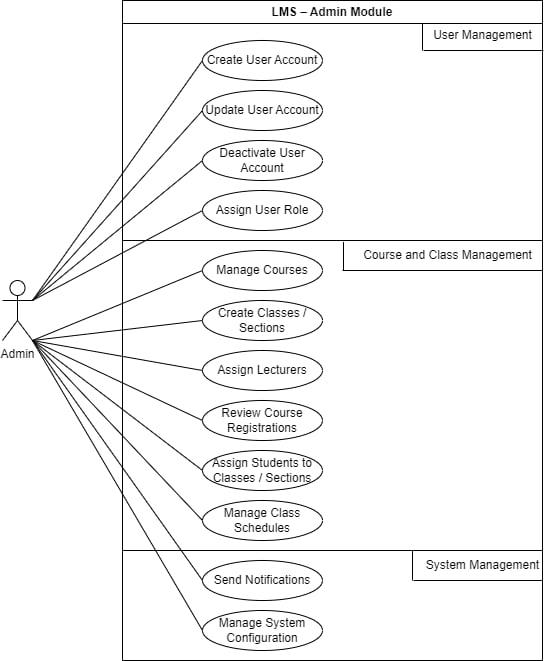
\includegraphics[width=0.8\textwidth, height=0.7\textheight, keepaspectratio]{images/usecase/AdminUsecase.png}
    \caption{Admin Use Case Diagram}
    \label{fig:admin-usecase}
\end{figure}


% ==========================================
% Admin Use Case Descriptions
% ==========================================

\renewcommand{\arraystretch}{1.1}
\setlength{\tabcolsep}{8pt}

% ==========================================
% UC-ADM-01: Create User Account
% ==========================================
\begin{longtable}{|>{\bfseries\raggedright\arraybackslash}p{0.205\textwidth}|>{\raggedright\arraybackslash}p{0.70\textwidth}|}
\hline
Use-case ID & UC-ADM-01 \\ \hline
Use-case name & Create User Account \\ \hline
Author & [Author Name] \\ \hline
Description & Allows the administrator to create a new user account by entering the required information and assigning a mandatory role to the account. \\ \hline
Actor & System Administrator \\ \hline
Trigger & The System Administrator selects the create user account function. \\ \hline
Precondition &
1. The System Administrator has a valid, active account. \par
2. The System Administrator has successfully logged in. \par
3. The system's user management service is available. \\ \hline
Postcondition & A new user account is created successfully with the assigned role and is stored in the system. \\ \hline
Normal Flow &
1. The System Administrator opens the user management module. \par
2. The System Administrator selects the create user account function. \par
3. The system displays the user creation form. \par
4. The System Administrator enters the required user information. \par
5. The System Administrator selects a role for the new account: Student, Lecturer, or Admin. \par
6. The system validates the submitted information and checks whether the selected role is valid. \par
7. The system creates the new account and assigns the selected role. \par
8. The system displays a confirmation message. \\ \hline
Alternative Flow &
\textbf{A1: Create an account with a different role} \par
1. At step 5, the System Administrator selects another available role. \par
2. The system updates the selected role in the creation form. \par
3. The System Administrator continues with step 6 of the normal flow. \\ \hline
Exception Flow &
\textbf{E1: Missing required information} \par
1. At step 6 of the normal flow, the system detects missing required information. \par
2. The system displays validation errors and requests the System Administrator to complete the missing fields. \par\vspace{4pt}
\textbf{E2: Role not selected or invalid role} \par
1. At step 6 of the normal flow, the system detects that no role has been selected or the selected role is invalid. \par
2. The system rejects the submission and requests a valid role selection. \par\vspace{4pt}
\textbf{E3: Account already exists} \par
1. At step 6 of the normal flow, the system detects that the account information conflicts with an existing account. \par
2. The system displays an error message and requests different account information. \\ \hline
\end{longtable}


% ==========================================
% UC-ADM-02: Update User Account
% ==========================================
\begin{longtable}{|>{\bfseries\raggedright\arraybackslash}p{0.205\textwidth}|>{\raggedright\arraybackslash}p{0.70\textwidth}|}
\hline
Use-case ID & UC-ADM-02 \\ \hline
Use-case name & Update User Account \\ \hline
Author & [Author Name] \\ \hline
Description & Allows the administrator to view and update the information of an existing user account. \\ \hline
Actor & System Administrator \\ \hline
Trigger & The System Administrator selects a user account to update. \\ \hline
Precondition &
1. The System Administrator has successfully logged in. \par
2. The System Administrator has the required administrative permissions. \par
3. The selected user account exists in the system. \\ \hline
Postcondition & The selected user account information is updated successfully, and the changes are stored in the system. \\ \hline
Normal Flow &
1. The System Administrator opens the user management module. \par
2. The system displays the available user accounts. \par
3. The System Administrator searches for and selects a user account. \par
4. The system displays the selected account's information. \par
5. The System Administrator modifies the required information. \par
6. The system validates the updated information. \par
7. The system saves the changes. \par
8. The system displays a confirmation message. \\ \hline
Alternative Flow &
\textbf{A1: View user account information} \par
1. At step 4, the System Administrator chooses to view the account without making changes. \par
2. The system displays the account information. \par
3. The use case ends without modifying the account. \\ \hline
Exception Flow &
\textbf{E1: User account not found} \par
1. At step 3 of the normal flow, the system cannot find the selected account. \par
2. The system displays a notification that the account does not exist. \par\vspace{4pt}
\textbf{E2: Invalid account information} \par
1. At step 6 of the normal flow, the system detects missing or invalid information. \par
2. The system displays validation errors and requests corrections. \par\vspace{4pt}
\textbf{E3: Update failure} \par
1. At step 7 of the normal flow, the system cannot save the changes. \par
2. The system displays an error message and retains the previous account information. \\ \hline
\end{longtable}


% ==========================================
% UC-ADM-03: Deactivate User Account
% ==========================================
\begin{longtable}{|>{\bfseries\raggedright\arraybackslash}p{0.205\textwidth}|>{\raggedright\arraybackslash}p{0.70\textwidth}|}
\hline
Use-case ID & UC-ADM-03 \\ \hline
Use-case name & Deactivate User Account \\ \hline
Author & [Author Name] \\ \hline
Description & Allows the administrator to deactivate an existing user account without permanently deleting it, preventing the user from logging in while preserving the account's data and learning history. \\ \hline
Actor & System Administrator \\ \hline
Trigger & The System Administrator selects the deactivate account function for a user. \\ \hline
Precondition &
1. The System Administrator has successfully logged in. \par
2. The System Administrator has the required administrative permissions. \par
3. The selected user account exists and is currently active. \\ \hline
Postcondition & The selected account is deactivated, the user can no longer log in, and all associated data and learning history are preserved. \\ \hline
Normal Flow &
1. The System Administrator opens the user management module. \par
2. The System Administrator searches for and selects a user account. \par
3. The system displays the account information and current status. \par
4. The System Administrator selects the deactivate account function. \par
5. The system requests confirmation of the operation. \par
6. The System Administrator confirms the deactivation. \par
7. The system changes the account status to inactive. \par
8. The system prevents the deactivated user from logging in. \par
9. The system preserves the account's associated data and learning history. \par
10. The system displays a confirmation message. \\ \hline
Alternative Flow &
\textbf{A1: Cancel account deactivation} \par
1. At step 5, the System Administrator chooses to cancel the operation. \par
2. The system keeps the account active. \par
3. The use case ends without modifying the account status. \\ \hline
Exception Flow &
\textbf{E1: Account not found} \par
1. At step 2 of the normal flow, the system cannot find the selected account. \par
2. The system displays an account not found message. \par\vspace{4pt}
\textbf{E2: Account already inactive} \par
1. At step 3 of the normal flow, the system detects that the account is already inactive. \par
2. The system informs the System Administrator that no deactivation is required. \par\vspace{4pt}
\textbf{E3: Deactivation failure} \par
1. At step 7 of the normal flow, the system cannot update the account status. \par
2. The system displays an error message and retains the previous account status. \\ \hline
\end{longtable}


% ==========================================
% UC-ADM-04: Assign User Role
% ==========================================
\begin{longtable}{|>{\bfseries\raggedright\arraybackslash}p{0.205\textwidth}|>{\raggedright\arraybackslash}p{0.70\textwidth}|}
\hline
Use-case ID & UC-ADM-04 \\ \hline
Use-case name & Assign User Role \\ \hline
Author & [Author Name] \\ \hline
Description & Allows the administrator to assign or change a user's role among Student, Lecturer, and Admin according to the system's access control rules. \\ \hline
Actor & System Administrator \\ \hline
Trigger & The System Administrator selects the role assignment function for a user account. \\ \hline
Precondition &
1. The System Administrator has successfully logged in. \par
2. The System Administrator has the required administrative permissions. \par
3. The selected user account exists in the system. \\ \hline
Postcondition & The selected user account is assigned the new valid role, and the role information is updated in the system. \\ \hline
Normal Flow &
1. The System Administrator opens the user management module. \par
2. The System Administrator selects a user account. \par
3. The system displays the account information and current role. \par
4. The System Administrator selects the assign or change role function. \par
5. The system displays the available roles: Student, Lecturer, and Admin. \par
6. The System Administrator selects the required role. \par
7. The system validates the selected role and checks the administrator's permissions. \par
8. The system updates the user's role. \par
9. The system applies the corresponding access permissions. \par
10. The system displays a confirmation message. \\ \hline
Alternative Flow &
\textbf{A1: Keep the current role} \par
1. At step 6, the System Administrator chooses to retain the existing role. \par
2. The system makes no changes to the account's role. \par
3. The use case ends. \\ \hline
Exception Flow &
\textbf{E1: User account not found} \par
1. At step 2 of the normal flow, the system cannot find the selected account. \par
2. The system displays an account not found message. \par\vspace{4pt}
\textbf{E2: Invalid role selection} \par
1. At step 7 of the normal flow, the system detects a role that is not supported by the system. \par
2. The system rejects the role assignment and requests a valid selection. \par\vspace{4pt}
\textbf{E3: Role update failure} \par
1. At step 8 of the normal flow, the system cannot save the new role. \par
2. The system displays an error message and retains the previous role. \\ \hline
\end{longtable}


% ==========================================
% UC-ADM-05: Manage Courses
% ==========================================
\begin{longtable}{|>{\bfseries\raggedright\arraybackslash}p{0.205\textwidth}|>{\raggedright\arraybackslash}p{0.70\textwidth}|}
\hline
Use-case ID & UC-ADM-05 \\ \hline
Use-case name & Manage Courses \\ \hline
Author & [Author Name] \\ \hline
Description & Allows the administrator to create, view, update, and deactivate courses in the learning management system. \\ \hline
Actor & System Administrator \\ \hline
Trigger & The System Administrator accesses the course management module. \\ \hline
Precondition &
1. The System Administrator has successfully logged in. \par
2. The System Administrator has the required administrative permissions. \par
3. The course management service is available. \\ \hline
Postcondition & Course information is created or updated successfully, or the selected course is deactivated while its associated data is preserved. \\ \hline
Normal Flow &
1. The System Administrator opens the course management module. \par
2. The system displays the available courses and management functions. \par
3. The System Administrator selects an operation, such as creating, viewing, updating, or deactivating a course. \par
4. The System Administrator enters or modifies the required course information. \par
5. The system validates the submitted information. \par
6. The system saves the new or updated course information, or changes the course status to inactive when deactivation is selected. \par
7. The system preserves associated course records when a course is deactivated. \par
8. The system displays a confirmation message. \\ \hline
Alternative Flow &
\textbf{A1: View course information} \par
1. At step 3, the System Administrator selects a course to view. \par
2. The system displays the course details and current status. \par
3. The use case ends without modifying the course. \par\vspace{4pt}
\textbf{A2: Cancel course deactivation} \par
1. At step 3, the System Administrator selects the deactivation function but cancels the confirmation. \par
2. The system keeps the course active. \\ \hline
Exception Flow &
\textbf{E1: Invalid course information} \par
1. At step 5 of the normal flow, the system detects missing or invalid course information. \par
2. The system displays validation errors and requests corrections. \par\vspace{4pt}
\textbf{E2: Course not found} \par
1. At step 3 of the normal flow, the system cannot find the selected course. \par
2. The system displays a course not found message. \par\vspace{4pt}
\textbf{E3: Course update failure} \par
1. At step 6 of the normal flow, the system cannot save the changes. \par
2. The system displays an error message and retains the previous course information and status. \\ \hline
\end{longtable}


% ==========================================
% UC-ADM-06: Create Classes or Sections
% ==========================================
\begin{longtable}{|>{\bfseries\raggedright\arraybackslash}p{0.205\textwidth}|>{\raggedright\arraybackslash}p{0.70\textwidth}|}
\hline
Use-case ID & UC-ADM-06 \\ \hline
Use-case name & Create Classes or Sections \\ \hline
Author & [Author Name] \\ \hline
Description & Allows the administrator to create a class or section associated with an existing course. \\ \hline
Actor & System Administrator \\ \hline
Trigger & The System Administrator selects the create class or section function. \\ \hline
Precondition &
1. The System Administrator has successfully logged in. \par
2. The System Administrator has the required administrative permissions. \par
3. The associated course exists and is active. \\ \hline
Postcondition & A new class or section is created and associated with the selected course. \\ \hline
Normal Flow &
1. The System Administrator opens the class management module. \par
2. The System Administrator selects the create class or section function. \par
3. The system displays the class creation form and available courses. \par
4. The System Administrator selects an existing course. \par
5. The System Administrator enters the required class or section information. \par
6. The system validates the submitted information and verifies the selected course. \par
7. The system creates the class or section and associates it with the selected course. \par
8. The system displays a confirmation message. \\ \hline
Alternative Flow &
\textbf{A1: Select another course} \par
1. At step 4, the System Administrator selects a different available course. \par
2. The system updates the selected course in the form. \par
3. The System Administrator continues with step 5 of the normal flow. \\ \hline
Exception Flow &
\textbf{E1: Course not found or inactive} \par
1. At step 6 of the normal flow, the system detects that the selected course does not exist or is inactive. \par
2. The system rejects the creation request and asks the System Administrator to select an active course. \par\vspace{4pt}
\textbf{E2: Invalid class information} \par
1. At step 6 of the normal flow, the system detects missing or invalid class information. \par
2. The system displays validation errors and requests corrections. \par\vspace{4pt}
\textbf{E3: Class creation failure} \par
1. At step 7 of the normal flow, the system cannot create the class or section. \par
2. The system displays an error message and allows the System Administrator to retry. \\ \hline
\end{longtable}


% ==========================================
% UC-ADM-07: Assign Lecturers
% ==========================================
\begin{longtable}{|>{\bfseries\raggedright\arraybackslash}p{0.205\textwidth}|>{\raggedright\arraybackslash}p{0.70\textwidth}|}
\hline
Use-case ID & UC-ADM-07 \\ \hline
Use-case name & Assign Lecturers \\ \hline
Author & [Author Name] \\ \hline
Description & Allows the administrator to assign eligible lecturers to classes or courses while ensuring that the selected lecturer has the correct role and no scheduling conflicts. \\ \hline
Actor & System Administrator \\ \hline
Trigger & The System Administrator selects the lecturer assignment function for a class or course. \\ \hline
Precondition &
1. The System Administrator has successfully logged in. \par
2. The selected course and class or section exist and are active. \par
3. At least one active lecturer account is available in the system. \\ \hline
Postcondition & An eligible lecturer is assigned to the selected class or course without violating the scheduling constraints. \\ \hline
Normal Flow &
1. The System Administrator opens the class or course management module. \par
2. The System Administrator selects a class or course. \par
3. The System Administrator selects the assign lecturer function. \par
4. The system displays eligible lecturer accounts. \par
5. The System Administrator selects a lecturer. \par
6. The system verifies that the selected account is active and has the Lecturer role. \par
7. The system checks whether the lecturer is eligible to teach the selected course. \par
8. The system checks for scheduling conflicts involving the lecturer. \par
9. The system assigns the lecturer to the selected class or course. \par
10. The system displays a confirmation message. \\ \hline
Alternative Flow &
\textbf{A1: Select another lecturer} \par
1. At step 5, the System Administrator selects a different lecturer. \par
2. The system performs the eligibility and scheduling checks for the newly selected lecturer. \par
3. The System Administrator continues with the assignment process. \\ \hline
Exception Flow &
\textbf{E1: Invalid lecturer account} \par
1. At step 6 of the normal flow, the system detects that the selected account is inactive or does not have the Lecturer role. \par
2. The system rejects the assignment and requests another eligible lecturer. \par\vspace{4pt}
\textbf{E2: Lecturer not eligible for the course} \par
1. At step 7 of the normal flow, the system determines that the lecturer is not associated with or eligible to teach the selected course. \par
2. The system rejects the assignment and displays an appropriate message. \par\vspace{4pt}
\textbf{E3: Lecturer scheduling conflict} \par
1. At step 8 of the normal flow, the system detects a time conflict with another assigned class. \par
2. The system rejects the assignment and informs the System Administrator of the conflict. \par\vspace{4pt}
\textbf{E4: Assignment failure} \par
1. At step 9 of the normal flow, the system cannot save the lecturer assignment. \par
2. The system displays an error message and leaves the previous assignment unchanged. \\ \hline
\end{longtable}


% ==========================================
% UC-ADM-08: Review Course Registrations
% ==========================================
\begin{longtable}{|>{\bfseries\raggedright\arraybackslash}p{0.205\textwidth}|>{\raggedright\arraybackslash}p{0.70\textwidth}|}
\hline
Use-case ID & UC-ADM-08 \\ \hline
Use-case name & Review Course Registrations \\ \hline
Author & [Author Name] \\ \hline
Description & Allows the administrator to review student course registration requests and approve or reject them. \\ \hline
Actor & System Administrator \\ \hline
Trigger & The System Administrator opens the course registration management module. \\ \hline
Precondition &
1. The System Administrator has successfully logged in. \par
2. The System Administrator has the required administrative permissions. \par
3. Student course registration requests are available for review. \\ \hline
Postcondition & The selected registration request is approved or rejected, and its status is updated in the system. \\ \hline
Normal Flow &
1. The System Administrator opens the course registration management module. \par
2. The system displays pending student registration requests. \par
3. The System Administrator selects a registration request. \par
4. The system displays the student's information and requested course. \par
5. The System Administrator reviews the registration information. \par
6. The System Administrator chooses to approve or reject the request. \par
7. The system validates the request and updates its registration status. \par
8. The system records the decision. \par
9. The system displays a confirmation message. \\ \hline
Alternative Flow &
\textbf{A1: Approve a registration request} \par
1. At step 6, the System Administrator selects approve. \par
2. The system changes the registration status to approved. \par
3. The approved registration becomes eligible for the subsequent class assignment process. \par\vspace{4pt}
\textbf{A2: Reject a registration request} \par
1. At step 6, the System Administrator selects reject. \par
2. The system changes the registration status to rejected. \par
3. The system records the decision. \\ \hline
Exception Flow &
\textbf{E1: Registration request not found} \par
1. At step 3 of the normal flow, the system cannot find the selected registration request. \par
2. The system displays a notification that the request is unavailable. \par\vspace{4pt}
\textbf{E2: Request already processed} \par
1. At step 7 of the normal flow, the system detects that the request has already been approved or rejected. \par
2. The system informs the System Administrator of the current request status. \par\vspace{4pt}
\textbf{E3: Registration update failure} \par
1. At step 7 of the normal flow, the system cannot update the registration status. \par
2. The system displays an error message and retains the previous status. \\ \hline
\end{longtable}


% ==========================================
% UC-ADM-09: Assign Students to Classes or Sections
% ==========================================
\begin{longtable}{|>{\bfseries\raggedright\arraybackslash}p{0.205\textwidth}|>{\raggedright\arraybackslash}p{0.70\textwidth}|}
\hline
Use-case ID & UC-ADM-09 \\ \hline
Use-case name & Assign Students to Classes or Sections \\ \hline
Author & [Author Name] \\ \hline
Description & Allows the administrator to assign eligible students to classes or sections after their course registration has been approved. \\ \hline
Actor & System Administrator \\ \hline
Trigger & The System Administrator selects the assign students function for a class or section. \\ \hline
Precondition &
1. The System Administrator has successfully logged in. \par
2. The selected course and class or section exist and are active. \par
3. The student has an active account with the Student role. \par
4. The student's registration for the selected course has been approved. \\ \hline
Postcondition & The eligible student is assigned to the selected class or section without duplicate enrollment. \\ \hline
Normal Flow &
1. The System Administrator opens the class management module. \par
2. The System Administrator selects a course and its class or section. \par
3. The System Administrator selects the assign students function. \par
4. The system displays students with approved registration for the selected course. \par
5. The System Administrator selects a student. \par
6. The system verifies that the student's account is active and has the Student role. \par
7. The system verifies that the student's course registration has been approved. \par
8. The system checks whether the student is already assigned to the selected class or section. \par
9. The system assigns the student to the class or section. \par
10. The system displays a confirmation message. \\ \hline
Alternative Flow &
\textbf{A1: Assign multiple students} \par
1. At step 5, the System Administrator selects multiple eligible students. \par
2. The system validates each selected student's eligibility. \par
3. The system assigns the eligible students to the selected class or section. \par
4. The system displays the assignment results. \\ \hline
Exception Flow &
\textbf{E1: Invalid student account} \par
1. At step 6 of the normal flow, the system detects that the selected account is inactive or does not have the Student role. \par
2. The system rejects the assignment. \par\vspace{4pt}
\textbf{E2: Course registration not approved} \par
1. At step 7 of the normal flow, the system detects that the student's registration has not been approved. \par
2. The system rejects the assignment and informs the System Administrator. \par\vspace{4pt}
\textbf{E3: Duplicate class assignment} \par
1. At step 8 of the normal flow, the system detects that the student is already assigned to the selected class or section. \par
2. The system prevents duplicate assignment and displays a notification. \par\vspace{4pt}
\textbf{E4: Assignment failure} \par
1. At step 9 of the normal flow, the system cannot save the assignment. \par
2. The system displays an error message and allows the System Administrator to retry. \\ \hline
\end{longtable}


% ==========================================
% UC-ADM-10: Manage Class Schedules
% ==========================================
\begin{longtable}{|>{\bfseries\raggedright\arraybackslash}p{0.205\textwidth}|>{\raggedright\arraybackslash}p{0.70\textwidth}|}
\hline
Use-case ID & UC-ADM-10 \\ \hline
Use-case name & Manage Class Schedules \\ \hline
Author & [Author Name] \\ \hline
Description & Allows the administrator to create and update class schedules while checking for conflicts involving time, room, lecturer, and assigned students. \\ \hline
Actor & System Administrator \\ \hline
Trigger & The System Administrator opens the class schedule management function. \\ \hline
Precondition &
1. The System Administrator has successfully logged in. \par
2. The System Administrator has the required administrative permissions. \par
3. The selected class or section exists in the system. \\ \hline
Postcondition & The class schedule is created or updated successfully without any detected scheduling conflicts. \\ \hline
Normal Flow &
1. The System Administrator opens the class schedule management module. \par
2. The System Administrator selects a class or section. \par
3. The system displays the current schedule, if available. \par
4. The System Administrator enters or modifies the schedule information, including time, room, and assigned lecturer. \par
5. The system validates the submitted schedule information. \par
6. The system checks for time conflicts involving the room, lecturer, and assigned students. \par
7. The system saves the schedule if no conflicts are detected. \par
8. The system displays a confirmation message. \\ \hline
Alternative Flow &
\textbf{A1: View an existing schedule} \par
1. At step 3, the System Administrator chooses to view the current schedule without modifying it. \par
2. The system displays the schedule details. \par
3. The use case ends without changing the schedule. \par\vspace{4pt}
\textbf{A2: Modify an existing schedule} \par
1. At step 4, the System Administrator updates an existing schedule. \par
2. The system validates the updated information and performs the conflict checks. \par
3. The System Administrator continues with step 7 of the normal flow if no conflicts are found. \\ \hline
Exception Flow &
\textbf{E1: Invalid schedule information} \par
1. At step 5 of the normal flow, the system detects missing or invalid schedule information. \par
2. The system displays validation errors and requests corrections. \par\vspace{4pt}
\textbf{E2: Scheduling conflict detected} \par
1. At step 6 of the normal flow, the system detects a conflict involving the schedule time, room, lecturer, or assigned students. \par
2. The system rejects the schedule change and identifies the detected conflict. \par\vspace{4pt}
\textbf{E3: Schedule update failure} \par
1. At step 7 of the normal flow, the system cannot save the schedule. \par
2. The system displays an error message and retains the previous valid schedule. \\ \hline
\end{longtable}


% ==========================================
% UC-ADM-11: Send Notifications
% ==========================================
\begin{longtable}{|>{\bfseries\raggedright\arraybackslash}p{0.205\textwidth}|>{\raggedright\arraybackslash}p{0.70\textwidth}|}
\hline
Use-case ID & UC-ADM-11 \\ \hline
Use-case name & Send Notifications \\ \hline
Author & [Author Name] \\ \hline
Description & Allows the administrator to send notifications to relevant users through the system's available notification channels. \\ \hline
Actor & System Administrator \\ \hline
Trigger & The System Administrator selects the send notification function. \\ \hline
Precondition &
1. The System Administrator has successfully logged in. \par
2. The System Administrator has the required administrative permissions. \par
3. The notification service is available. \\ \hline
Postcondition & The notification is created and submitted to the selected delivery channel or channels. \\ \hline
Normal Flow &
1. The System Administrator opens the notification management module. \par
2. The System Administrator selects the send notification function. \par
3. The system displays the notification form. \par
4. The System Administrator enters the notification title and content. \par
5. The System Administrator selects the intended recipients. \par
6. The System Administrator selects the available notification channels, such as in-system notifications or email. \par
7. The system validates the notification content and recipient information. \par
8. The system submits the notification through the selected channels. \par
9. The system displays a confirmation message. \\ \hline
Alternative Flow &
\textbf{A1: Send a notification to a specific group} \par
1. At step 5, the System Administrator selects a specific group of users, such as Students or Lecturers. \par
2. The system identifies the users belonging to the selected group. \par
3. The System Administrator continues with step 6 of the normal flow. \\ \hline
Exception Flow &
\textbf{E1: Invalid notification content} \par
1. At step 7 of the normal flow, the system detects missing or invalid notification information. \par
2. The system displays validation errors and requests corrections. \par\vspace{4pt}
\textbf{E2: No valid recipients} \par
1. At step 7 of the normal flow, the system determines that no valid recipients are available. \par
2. The system informs the System Administrator and does not send the notification. \par\vspace{4pt}
\textbf{E3: Notification delivery failure} \par
1. At step 8 of the normal flow, the system cannot submit the notification through one or more selected channels. \par
2. The system reports the delivery failure and displays the available delivery status. \\ \hline
\end{longtable}


% ==========================================
% UC-ADM-12: Manage System Configuration
% ==========================================
\begin{longtable}{|>{\bfseries\raggedright\arraybackslash}p{0.205\textwidth}|>{\raggedright\arraybackslash}p{0.70\textwidth}|}
\hline
Use-case ID & UC-ADM-12 \\ \hline
Use-case name & Manage System Configuration \\ \hline
Author & [Author Name] \\ \hline
Description & Allows the administrator to view and update configurable system settings according to the administrator's permissions. \\ \hline
Actor & System Administrator \\ \hline
Trigger & The System Administrator accesses the system configuration module. \\ \hline
Precondition &
1. The System Administrator has successfully logged in. \par
2. The System Administrator has the required administrative permissions. \par
3. The system configuration service is available. \\ \hline
Postcondition & The selected system configuration settings are updated successfully, and the changes are stored in the system. \\ \hline
Normal Flow &
1. The System Administrator opens the system configuration module. \par
2. The system displays the available configuration settings. \par
3. The System Administrator selects a setting to view or modify. \par
4. The system displays the current value of the selected setting. \par
5. The System Administrator enters the new configuration value. \par
6. The system validates the submitted value and checks the administrator's permissions. \par
7. The system saves the updated configuration. \par
8. The system records the change and displays a confirmation message. \\ \hline
Alternative Flow &
\textbf{A1: View configuration settings} \par
1. At step 3, the System Administrator chooses to view a setting without modifying it. \par
2. The system displays the current configuration value. \par
3. The use case ends without changing the configuration. \\ \hline
Exception Flow &
\textbf{E1: Invalid configuration value} \par
1. At step 6 of the normal flow, the system detects an invalid configuration value. \par
2. The system displays a validation error and requests a valid value. \par\vspace{4pt}
\textbf{E2: Insufficient permissions} \par
1. At step 6 of the normal flow, the system determines that the administrator does not have permission to modify the selected setting. \par
2. The system rejects the operation and displays an authorization error. \par\vspace{4pt}
\textbf{E3: Configuration update failure} \par
1. At step 7 of the normal flow, the system cannot save the configuration. \par
2. The system displays an error message and retains the previous valid configuration. \\ \hline
\end{longtable}


\subsubsection{Teacher use case}
\begin{figure}[H]
    \centering
    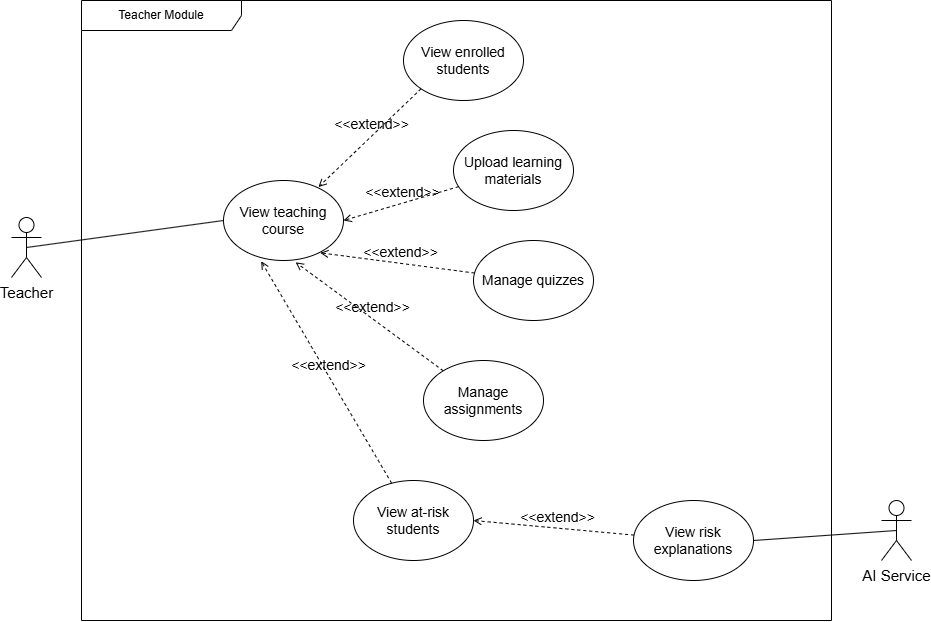
\includegraphics[width=0.8\textwidth, height=0.7\textheight, keepaspectratio]{images/usecase/teacher.png}
    \caption{Teacher Use Case Diagram}
    \label{fig:teacher-usecase}
\end{figure}

{
\renewcommand{\arraystretch}{1.1}
\setlength{\tabcolsep}{8pt}
\begin{longtable}{|>{\bfseries\raggedright\arraybackslash}p{0.205\textwidth}|>{\raggedright\arraybackslash}p{0.70\textwidth}|}
\hline
%--------------------------------------------------------------------------------
Use-case ID & UC-010 \\ \hline
%--------------------------------------------------------------------------------
Use-case name & View Teaching Course \\ \hline
%--------------------------------------------------------------------------------
Author & Thai Thien Hai Long \\ \hline
%--------------------------------------------------------------------------------
Description &
Allows the lecturer to view the Course Home Page and its overview dashboard. It serves as the central entry point for accessing learning materials, assessments, student rosters, and AI risk analytics.\\ \hline
%--------------------------------------------------------------------------------
Actor & Teacher \\ \hline
%--------------------------------------------------------------------------------
Trigger &
The teacher selects a specific course from their teaching course list on the dashboard. \\ \hline
%--------------------------------------------------------------------------------
Precondition &
1. The user is authenticated and logged in with the teacher role. \par
2. The user has been assigned to teach at least one active course by the admin. \\ \hline
%--------------------------------------------------------------------------------
Postcondition &
The course home page is displayed, presenting active course sections, announcements, and navigation links to course tools. \\ \hline
%--------------------------------------------------------------------------------
Normal Flow &
1. The teacher navigates to the ``My Courses'' section from the main navigation menu. \par
2. The system retrieves and displays the list of courses assigned to the teacher. \par
3. The teacher selects a specific course to inspect. \par
4. The system navigates to the course home page. \par
5. The system displays course sections, announcements, and existing learning materials.\\ \hline
%--------------------------------------------------------------------------------
Alternative Flow &
N/A. \\ \hline
%--------------------------------------------------------------------------------
Exception Flow &
\textbf{E1: No Assigned Courses Found} \par
1. At step 2 of the normal flow, no courses are assigned to the teacher's account. \par
2. The system displays a ``No courses'' placeholder. \par\vspace{4pt}
\textbf{E2: Course Load Failure} \par
1. At step 4 of the normal flow, the course fails to load due to a system error. \par
2. The system displays an error alert: ``Unable to load course. Please try again.'' \\ \hline
\end{longtable}
}

{
\renewcommand{\arraystretch}{1.1}
\setlength{\tabcolsep}{8pt}
\begin{longtable}{|>{\bfseries\raggedright\arraybackslash}p{0.205\textwidth}|>{\raggedright\arraybackslash}p{0.70\textwidth}|}
\hline
%--------------------------------------------------------------------------------
Use-case ID & UC-011 \\ \hline
%--------------------------------------------------------------------------------
Use-case name & View Enrolled Students \\ \hline
%--------------------------------------------------------------------------------
Author & Thai Thien Hai Long \\ \hline
%--------------------------------------------------------------------------------
Description &
Allows the teacher to view, filter, and monitor the enrolled student roster, including assigned groups and recent activity timestamps. \\ \hline
%--------------------------------------------------------------------------------
Actor & Teacher \\ \hline
%--------------------------------------------------------------------------------
Trigger &
The teacher clicks on the ``Participants'' tab from the course navigation bar. \\ \hline
%--------------------------------------------------------------------------------
Precondition &
1. The user is authenticated and logged in with the Teacher role.\par
2. The user has accessed the target course home page. \\ \hline
%--------------------------------------------------------------------------------
Postcondition &
The enrolled student roster is displayed, including student IDs, full names, assigned groups, and last access timestamps. \\ \hline
%--------------------------------------------------------------------------------
Normal Flow &
1. From the course home page, the teacher selects the ``Participants'' tab.\par
2. The system queries the database for all enrolled users associated with the course.\par
3. The system displays the participant table containing student names, ID numbers, email addresses, assigned groups, roles, and last access timestamps. \\ \hline
%--------------------------------------------------------------------------------
Alternative Flow &
\textbf{A1: Filter or Search Students}\par
1. At step 3 of the normal flow, the teacher enters a search keyword or selects a class group filter. \par
2. The system filters and displays the matching subset of enrolled students. \\ \hline
%--------------------------------------------------------------------------------
Exception Flow &
\textbf{E1: No Students Enrolled}\par
1. At step 2 of the normal flow, no student records are linked to the course.\par
2. The system displays an empty-state message: ``No participants found in this course.''\par\vspace{4pt}
\textbf{E2: Participant Data Load Failure}\par
1. At step 2 of the normal flow, the participant list fails to load due to a database connection error.\par
2. The system displays an error alert: ``Unable to retrieve participant list. Please refresh the page.'' \\ \hline
%--------------------------------------------------------------------------------
\end{longtable}
}

{
\renewcommand{\arraystretch}{1.1}
\setlength{\tabcolsep}{8pt}
\begin{longtable}{|>{\bfseries\raggedright\arraybackslash}p{0.21\textwidth}|>{\raggedright\arraybackslash}p{0.70\textwidth}|}
\hline
%--------------------------------------------------------------------------------
Use-case ID & UC-012 \\ \hline
%--------------------------------------------------------------------------------
Use-case name & Upload Learning Materials \\ \hline
%--------------------------------------------------------------------------------
Author & Thai Thien Hai Long \\ \hline
%--------------------------------------------------------------------------------
Description &
Allows the teacher to add learning resources (e.g., lecture slides, documents, syllabus, or links) to specific course sections for enrolled students to access. \\ \hline
%--------------------------------------------------------------------------------
Actor & Teacher \\ \hline
%--------------------------------------------------------------------------------
Trigger &
The teacher enables edit mode and selects ``Add an activity or resource'' within a course section. \\ \hline
%--------------------------------------------------------------------------------
Precondition &
1. The user is authenticated and logged in with the Teacher role. \par
2. The user has accessed the target course home page. \\ \hline
%--------------------------------------------------------------------------------
Postcondition &
The uploaded learning material is saved and displayed within the selected course section. \\ \hline
%--------------------------------------------------------------------------------
Normal Flow &
1. From the course home page, the teacher turns on ``Edit mode''. \par
2. In the target section, the teacher clicks ``Add an activity or resource'' and selects ``File'' (or ``Folder''). \par
3. The system displays the resource setup form. \par
4. The teacher inputs the resource name, description, and uploads the file attachment. \par
5. The teacher clicks ``Save and return to course''. \par
6. The system validates the file, stores it, and displays the new resource link in the course section. \\ \hline
%--------------------------------------------------------------------------------
Alternative Flow &
\textbf{A1: Upload via Drag-and-Drop} \par
1. At step 2 of the normal flow, the teacher directly drags and drops a file from the local file explorer into the desired section on the course page. \par
2. The system automatically uploads the file and creates a resource entry using the filename. \par\vspace{4pt}
\textbf{A2: Add External URL Resource} \par
1. At step 2 of the normal flow, the teacher selects ``URL'' instead of ``File''. \par
2. The teacher enters the resource title and external web address. \par
3. The flow proceeds to step 5. \\ \hline
%--------------------------------------------------------------------------------
Exception Flow &
\textbf{E1: File Size Exceeds Limit} \par
1. At step 5 of the normal flow, the uploaded file exceeds the course upload size limit. \par
2. The system rejects the file and displays an alert: ``The file is too large to be uploaded.'' \par
3. The flow returns to step 4 for file re-selection. \par\vspace{4pt}
\textbf{E2: Unsupported File Format} \par
1. At step 5 of the normal flow, the file format is restricted by system policy. \par
2. The system displays an error: ``This file type is not allowed.'' \par
3. The flow returns to step 4. \\ \hline
\end{longtable}
}

{
\renewcommand{\arraystretch}{1.1}
\setlength{\tabcolsep}{8pt}
\begin{longtable}{|>{\bfseries\raggedright\arraybackslash}p{0.21\textwidth}|>{\raggedright\arraybackslash}p{0.70\textwidth}|}
\hline
%--------------------------------------------------------------------------------
Use-case ID & UC-013 \\ \hline
%--------------------------------------------------------------------------------
Use-case name & Manage Quizzes \\ \hline
%--------------------------------------------------------------------------------
Author & Thai Thien Hai Long \\ \hline
%--------------------------------------------------------------------------------
Description &
Allows the teacher to create, configure, update, or remove online quiz assessments and define question sets and grading rules for the course. \\ \hline
%--------------------------------------------------------------------------------
Actor & Teacher \\ \hline
%--------------------------------------------------------------------------------
Trigger &
The teacher enables edit mode and selects ``Add an activity or resource'' > ``Quiz'' within a course section. \\ \hline
%--------------------------------------------------------------------------------
Precondition &
1. The user is authenticated and logged in with the Teacher role. \par
2. The user has accessed the target course home page. \\ \hline
%--------------------------------------------------------------------------------
Postcondition &
The quiz activity and its configured question items are saved and published in the designated course section. \\ \hline
%--------------------------------------------------------------------------------
Normal Flow &
1. From the course home page, the teacher turns on ``Edit mode''. \par
2. In the target section, the teacher clicks ``Add an activity or resource'' and selects ``Quiz''. \par
3. The system displays the quiz settings page (timing, grade boundaries, attempt limits). \par
4. The teacher configures the quiz parameters and clicks ``Save and display''. \par
5. The system opens the quiz question management interface. \par
6. The teacher adds questions from the question bank or creates new questions with point values. \par
7. The teacher saves the assessment. \par
8. The system updates the quiz structure and makes it accessible in the course section. \\ \hline
%--------------------------------------------------------------------------------
Alternative Flow &
\textbf{A1: Edit Existing Quiz} \par
1. At step 2 of the normal flow, the teacher clicks the action menu of an existing quiz and selects ``Edit settings''. \par
2. The system loads existing configurations and questions. \par
3. The teacher updates parameters or modifies questions. \par
4. The flow proceeds to step 7. \par\vspace{4pt}
\textbf{A2: Delete Quiz} \par
1. At step 2 of the normal flow, the teacher selects ``Delete'' on an existing quiz. \par
2. The system requests confirmation. \par
3. The teacher confirms deletion, and the system removes the quiz activity from the course. \\ \hline
%--------------------------------------------------------------------------------
Exception Flow &
\textbf{E1: Invalid Time Window} \par
1. At step 4 of the normal flow, the quiz close time is configured before the open time. \par
2. The system displays a validation error: ``The closing time cannot be earlier than the opening time.'' \par
3. The teacher adjusts the timestamps. \par\vspace{4pt}
\textbf{E2: Empty Question Set} \par
1. At step 7 of the normal flow, the teacher attempts to publish a quiz without adding any questions. \par
2. The system displays a warning notice: ``No questions have been added yet.'' \\ \hline
\end{longtable}
}

{
\renewcommand{\arraystretch}{1.1}
\setlength{\tabcolsep}{8pt}
\begin{longtable}{|>{\bfseries\raggedright\arraybackslash}p{0.21\textwidth}|>{\raggedright\arraybackslash}p{0.70\textwidth}|}
\hline
%--------------------------------------------------------------------------------
Use-case ID & UC-014 \\ \hline
%--------------------------------------------------------------------------------
Use-case name & Manage Assignments \\ \hline
%--------------------------------------------------------------------------------
Author & Thai Thien Hai Long \\ \hline
%--------------------------------------------------------------------------------
Description &
Allows the teacher to create, configure, update, or remove student assignment dropboxes, specifying submission formats, deadlines, and grading criteria. \\ \hline
%--------------------------------------------------------------------------------
Actor & Teacher \\ \hline
%--------------------------------------------------------------------------------
Trigger &
The teacher enables edit mode and selects ``Add an activity or resource'' > ``Assignment'' within a course section. \\ \hline
%--------------------------------------------------------------------------------
Precondition &
1. The user is authenticated and logged in with the Teacher role. \par
2. The user has accessed the target course home page. \\ \hline
%--------------------------------------------------------------------------------
Postcondition &
The assignment entry is created or updated, providing an active submission portal for enrolled students. \\ \hline
%--------------------------------------------------------------------------------
Normal Flow &
1. From the course home page, the teacher turns on ``Edit mode''. \par
2. In the target section, the teacher clicks ``Add an activity or resource'' and selects ``Assignment''. \par
3. The system displays the assignment configuration form. \par
4. The teacher specifies assignment title, description instructions, and optional prompt attachments. \par
5. The teacher configures availability dates (allow submissions from, due date, cutoff date) and file submission limits. \par
6. The teacher clicks ``Save and return to course''. \par
7. The system validates the submission parameters and publishes the assignment item. \\ \hline
%--------------------------------------------------------------------------------
Alternative Flow &
\textbf{A1: Edit Existing Assignment} \par
1. At step 2 of the normal flow, the teacher clicks the action menu of an existing assignment and selects ``Edit settings''. \par
2. The system populates the form with existing assignment configurations. \par
3. The teacher updates instructions or extends deadlines. \par
4. The flow proceeds to step 6. \par\vspace{4pt}
\textbf{A2: Delete Assignment} \par
1. At step 2 of the normal flow, the teacher selects ``Delete'' on an existing assignment. \par
2. The system prompts a confirmation dialog. \par
3. The teacher confirms deletion, and the system removes the assignment. \\ \hline
%--------------------------------------------------------------------------------
Exception Flow &
\textbf{E1: Invalid Due Date} \par
1. At step 6 of the normal flow, the specified due date precedes the allowable submission start date. \par
2. The system halts submission and displays an error: ``Due date must be after the allow submissions from date.'' \par
3. The flow returns to step 5. \par\vspace{4pt}
\textbf{E2: File Size Exceeds Limit} \par
1. At step 4 of the normal flow, the attached assignment prompt file exceeds maximum upload size. \par
2. The system rejects the file and displays an error alert: ``The uploaded instruction file exceeds size limits.'' \\ \hline
\end{longtable}
}

{
\renewcommand{\arraystretch}{1.1}
\setlength{\tabcolsep}{8pt}
\begin{longtable}{|>{\bfseries\raggedright\arraybackslash}p{0.21\textwidth}|>{\raggedright\arraybackslash}p{0.70\textwidth}|}
\hline
%--------------------------------------------------------------------------------
Use-case ID & UC-015 \\ \hline
%--------------------------------------------------------------------------------
Use-case name & View At-Risk Students and Risk Explanations \\ \hline
%--------------------------------------------------------------------------------
Author & Thai Thien Hai Long \\ \hline
%--------------------------------------------------------------------------------
Description &
Allows the teacher to review an AI-analyzed roster of enrolled students at academic risk within a specific course, inspect feature-based explanations (e.g., inactivity duration, assignment delays, or quiz drop-offs), and trigger personalized outreach interventions. \\ \hline
%--------------------------------------------------------------------------------
Actor & Teacher, AI Service (Secondary) \\ \hline
%--------------------------------------------------------------------------------
Trigger &
The teacher navigates to the ``Analytics / At-Risk Students'' section from the course management dashboard. \\ \hline
%--------------------------------------------------------------------------------
Precondition &
1. The user is authenticated and logged in with the Teacher role. \par
2. The user has accessed a course they are actively assigned to teach. \par
3. The background feature extraction and AI prediction pipeline has processed current student activity and grade logs. \\ \hline
%--------------------------------------------------------------------------------
Postcondition &
The teacher reviews categorized student risk profiles and explanations, and optional intervention actions (e.g., outreach email logs) are recorded. \\ \hline
%--------------------------------------------------------------------------------
Normal Flow &
1. From the course home page, the teacher navigates to the ``At-Risk Students'' analytics overview. \par
2. The system queries the AI service and displays the student roster categorized into risk levels (\textit{High Risk}, \textit{Medium Risk}, \textit{Safe}). \par
3. The teacher filters or sorts the roster by risk severity or student identifier. \par
4. The teacher selects a flagged student to view detailed risk indicators. \par
5. The system requests the explanation payload from the AI service. \par
6. The AI service computes/retrieves feature attributions and returns plain-language pedagogical reasons (e.g., prolonged inactivity, negative quiz score slopes, missing submissions). \par
7. The system renders the student risk profile along with the primary contributing factors and impact weights. \par
8. The teacher reviews the assessment and closes or acknowledges the report. \\ \hline
%--------------------------------------------------------------------------------
Alternative Flow &
\textbf{A1: Generate AI Intervention Outreach} \par
1. At step 7 of the normal flow, the teacher clicks ``Draft Personalized Outreach''. \par
2. The system prompts the generative AI service with the student's contributing risk factors to draft an empathetic email. \par
3. The teacher reviews, edits, and sends the drafted communication. \par
4. The system logs the intervention status and returns to step 3. \par\vspace{4pt}
\textbf{A2: Filter by Safe or Moderate Thresholds} \par
1. At step 3 of the normal flow, the teacher selects a filter to inspect stable or low-risk students. \par
2. The system updates the roster view to show students whose performance indicators meet course baselines. \\ \hline
%--------------------------------------------------------------------------------
Exception Flow &
\textbf{E1: Insufficient Activity Data for Evaluation} \par
1. At step 2 of the normal flow, the course has insufficient student interaction logs or submission records to compute reliable risk predictions. \par
2. The system displays an informational status banner: ``Insufficient activity data available to generate early warning predictions.'' \par
3. The flow terminates without rendering risk tiers. \par\vspace{4pt}
\textbf{E2: AI Service / Analytics Endpoint Unavailable} \par
1. At step 2 or step 5 of the normal flow, the connection to the AI analytics microservice times out or returns an error. \par
2. The system displays a notification alert: ``Unable to retrieve predictive analytics. Please try again later.'' \par
3. The system falls back to displaying raw gradebook summaries without AI risk classifications. \\ \hline
\end{longtable}
}


\chapter{Conclusion}

\input{sections/5.Conclusion/summary}
\renewcommand{\bibname}{References}
\addcontentsline{toc}{chapter}{References}
\nocite{*}
\printbibliography

\input{sections/appendixes/appendix}
\input{sections/appendixes/plan}
% add appendix later on

\end{document}
